% !TEX program = xelatex
\documentclass[10pt,letterpaper,twocolumn]{article}

% === GEOMETRY ===
% Bottom margin + footskip tuned so the page number sits ≥0.6in from the
% sheet edge — clear of consumer-inkjet unprintable zones (HP DeskJet
% bottom dead strip is 0.5in) without scaling the page down.
\usepackage[top=0.75in, bottom=0.75in, left=0.75in, right=0.75in, footskip=12pt]{geometry}

% === FONTS ===
\usepackage{fontspec}
\usepackage{unicode-math}
\usepackage{xeCJK}
\setCJKmainfont{Droid Sans Fallback}
\setmainfont{Latin Modern Roman}[
 Extension=.otf,
 UprightFont=lmroman10-regular,
 BoldFont=lmroman10-bold,
 ItalicFont=lmroman10-italic,
 BoldItalicFont=lmroman10-bolditalic,
]
% Droid Sans Fallback lacks em-dash / curly quotes / ellipsis; route these
% punctuation marks to the Latin Modern main font (which has them) so CJK
% prose renders no tofu.
\xeCJKDeclareCharClass{Default}{`—,`“,`”,`‘,`’,`…}
\setsansfont{Latin Modern Sans}[
 Extension=.otf,
 UprightFont=lmsans10-regular,
 BoldFont=lmsans10-bold,
 ItalicFont=lmsans10-oblique,
 BoldItalicFont=lmsans10-boldoblique,
]
\setmonofont{Latin Modern Mono}[
 Extension=.otf,
 UprightFont=lmmono10-regular,
 ItalicFont=lmmono10-italic,
 Scale=0.85,
]
% YWFT Processing is used in exactly ONE place: the title in the header.
% Its punctuation glyphs are unreliable (the "/" renders as an ampersand-
% like mark), so body text, subtitle, and the edition slot stay in the
% Latin Modern faces.
\newfontfamily\acbold{ywft-processing-bold}[
 Path=../../system/public/type/webfonts/,
 Extension=.ttf
]

% === PACKAGES ===
\usepackage{xcolor}
\usepackage{colortbl}
\usepackage{titlesec}
\usepackage{enumitem}
\usepackage{booktabs}
\usepackage{tabularx}
\usepackage{fancyhdr}
\usepackage{hyperref}
\usepackage{xurl}
\usepackage{graphicx}
\graphicspath{{./}{figures/}}
\usepackage{ragged2e}
\usepackage{microtype}
\usepackage[font=footnotesize]{caption}
\usepackage{afterpage}
\usepackage{multicol}
\usepackage{natbib}
\usepackage{tikz}
\usetikzlibrary{calc,positioning,shapes.geometric,arrows.meta}

% --- TikZ helpers for inline keyboard / hex / mapping diagrams ---
\definecolor{keyfill}{RGB}{248,248,250}
\definecolor{keystroke}{RGB}{160,156,170}
\definecolor{keymapped}{RGB}{180,72,135}
\definecolor{keysharp}{RGB}{52,52,64}
\tikzset{
 kcap/.style={draw=keystroke, fill=keyfill, rounded corners=0.6pt,
        minimum width=0.34cm, minimum height=0.34cm,
        inner sep=0pt, font=\scriptsize\sffamily},
 kcap mapped/.style={kcap, fill=keymapped!18, draw=keymapped!60,
            text=keymapped!90},
 kcap sharp/.style={kcap, fill=keysharp, draw=keysharp,
           text=white, font=\scriptsize\sffamily\bfseries},
 hexkey/.style={regular polygon, regular polygon sides=6,
         draw=keystroke, fill=keyfill, rounded corners=0pt,
         minimum size=0.55cm, inner sep=0pt,
         font=\tiny\sffamily},
 hexkey mapped/.style={hexkey, fill=keymapped!22, draw=keymapped!70,
             text=keymapped!90},
}
% === COLORS ===
\definecolor{acpink}{RGB}{180,72,135}
\definecolor{acpurple}{RGB}{120,80,180}
\definecolor{acdark}{RGB}{64,56,74}
\definecolor{acgray}{RGB}{119,119,119}
\definecolor{acblue}{RGB}{42,100,212}
\definecolor{acgreen}{RGB}{42,154,58}
\definecolor{acorange}{RGB}{216,120,0}
% Domain chip for the corollary table — small caps-ish bold colored tag
\newcommand{\dmn}[2]{\textcolor{#1}{\textbf{#2}}}
% Row QR code for the corollary table — links each object to its
% canonical home (Wikipedia, the project's own site, or its spec).
% PNGs generated by qrencode + magick PNG32 in figures/qr/.
% Centered on the row's text baseline so label text sits vertically
% centered against the tile.
\newcommand{\qrc}[1]{\raisebox{\dimexpr-0.5\height+0.8ex\relax}{\includegraphics[height=0.74cm]{figures/qr/#1.png}}}

% === HYPERREF ===
\hypersetup{
 colorlinks=true,
 linkcolor=acpurple,
 urlcolor=acpurple,
 citecolor=acpurple,
 pdfauthor={@jeffrey},
 pdftitle={作为社会软件的键位映射：经由社会契约的可版本化虚拟对象},
}

% === SECTION FORMATTING ===
\titleformat{\section}
 {\normalfont\bfseries\normalsize\uppercase}
 {\thesection.}
 {0.5em}
 {}
\titlespacing{\section}{0pt}{1.2em}{0.3em}

\titleformat{\subsection}
 {\normalfont\bfseries\small}
 {\thesubsection}
 {0.5em}
 {}
\titlespacing{\subsection}{0pt}{0.8em}{0.2em}

% === HEADER/FOOTER ===
\pagestyle{fancy}
\fancyhf{}
\renewcommand{\headrulewidth}{0pt}
\fancyfoot[C]{\footnotesize\thepage}
% Full-page table spread: folio moves to the bottom right so it can't
% collide with the table body.
\fancypagestyle{tablefolio}{%
 \fancyhf{}%
 \renewcommand{\headrulewidth}{0pt}%
 \fancyfoot[R]{\footnotesize\thepage}%
}

% === LIST SETTINGS ===
\setlist[itemize]{nosep, leftmargin=1.2em, itemsep=0.1em}
\setlist[enumerate]{nosep, leftmargin=1.2em}

% === COLUMN SEPARATION ===
\setlength{\columnsep}{1.8em}

% === PARAGRAPH SETTINGS ===
\setlength{\parindent}{1em}
\setlength{\parskip}{0.3em}

% Hyphenation for narrow two-column layout
\tolerance=800
\emergencystretch=1em
\hyphenpenalty=50

\newcommand{\acdot}{{\color{acpink}.}}
% Every dot in Aesthetic.Computer is the AC pink dot, inline too.
\newcommand{\ac}{Aesthetic{\acdot}Computer}
% Keycap chip — the one canonical inline key glyph: cap-height box
% (no descender slack, so it sits low in the text line) with a gray
% bottom-shadow bezel, like the keycaps in the figures.
\DeclareRobustCommand{\key}[1]{\tikz[baseline=(k.base)]{%
 \node[fill=keystroke, rounded corners=1.3pt, inner xsep=2.4pt,
    inner ysep=1.9pt, anchor=base, yshift=-1.2pt] at (0,0)
  {\footnotesize\ttfamily\bfseries\vphantom{A}\phantom{#1}};
 \node[draw=keystroke, line width=0.4pt, fill=keyfill,
    rounded corners=1.3pt, inner xsep=2.4pt, inner ysep=1.9pt,
    anchor=base] (k) at (0,0)
  {\footnotesize\ttfamily\bfseries\vphantom{A}#1};}}
% A run of keycaps with even spacing: \keys{C,D,E,F,G,A,B}
\makeatletter
\DeclareRobustCommand{\keys}[1]{{\def\sep{}\@for\kk:=#1\do{\sep\key{\kk}\def\sep{\,}}}}
\makeatother

% Version stamp (hash + revision). papers/cli.mjs regenerates
% version.tex from git on every build; the fallback defaults keep a
% manual `xelatex keymaps.tex` (no stamp present) compiling.
\InputIfFileExists{version}{}{%
 \providecommand{\paperhash}{dev}\providecommand{\paperrev}{?}}
\InputIfFileExists{history}{}{\providecommand{\paperhistory}{}}

% Cover language bar. The same paper is published in six languages; each
% edition links to the others by their canonical permalink. Language codes
% (not autonyms) keep the row legible in every font --- the Latin-only
% editions cannot render CJK/Cyrillic glyphs. \klanghere marks the current
% language; \klang links a sibling edition by its URL suffix ("" for en).
\newcommand{\klang}[2]{\href{https://papers.aesthetic.computer/keymaps-social-software-26-arxiv#2.pdf}{\color{acgray}#1}}
\newcommand{\klanghere}[1]{{\bfseries\color{acpink}#1}}
\newcommand{\klangsep}{{\color{acgray!60}\,\textperiodcentered\,}}

\begin{document}

\twocolumn[{%
\begin{center}
{\fontsize{27pt}{31pt}\selectfont\bfseries\color{acdark} 作为社会软件的键位映射}\par
\vspace{0.5em}

\includegraphics[width=0.7\textwidth]{figures/cover}\par
\vspace{0.4em}
{\itshape\fontsize{14.5pt}{17pt}\selectfont\color{acpink} 经由社会契约的可版本化虚拟对象}\par
\vspace{0.5em}
{\small\color{acgray} \href{https://prompt.ac/@jeffrey}{@jeffrey} \,$\cdot$\, Aesthetic{\acdot}Computer \,$\cdot$\, ORCID \href{https://orcid.org/0009-0007-4460-4913}{0009-0007-4460-4913}}\par
\vspace{0.45em}
{\footnotesize\sffamily\klang{EN}{}\klangsep\klang{DA}{-da}\klangsep\klang{ES}{-es}\klangsep\klanghere{ZH}\klangsep\klang{JA}{-ja}\klangsep\klang{RU}{-ru}}\par
\vspace{0.55em}
{\color{acpink}\rule{\textwidth}{1.2pt}}
\vspace{0.5em}
\end{center}

\begin{quote}
\small\noindent\textbf{摘要。}
一份\emph{键位映射}（keymap）——那张声明“QWERTY 键 \key{A} 弹奏 MIDI 60”的小型声明式表格——在每一种功能意义上都是软件：它被版本化、被发明、被分叉，并在各应用之间被需求。然而它不是二进制文件，不是项目，也不是服务，开源对专有的二分轴根本看不见它。我把这一范畴命名为\emph{社会软件}（social software）——既是对 Shirky 的一语双关，也接续了 McCarthy 与 Reas 在 UCLA 同名计划中的用法，本文正是在该计划之内写成——并自 Sholes 追溯至 Colemak、自 Jankó 追溯至 Wicki--Hayden，直至每一款主流 DAW 都附带的那套无人拥有的 QWERTY 钢琴约定——我依其前五个半音音级所落的按键，将其命名为 AWSED 布局。透过 Lialina 的《图灵完备的用户》~\citep{lialina2012turing}来读，键位映射正是用户可作者化的那道缝隙，其闭合即意味着用户作为作者的消失；我把 \texttt{notepat.com} 的键位映射——“为自己命名的音符”——作为这道缝隙仍然敞开的证据呈上。
\end{quote}
\vspace{0.5em}
}]

\section{引言：一件器物}

图~\ref{fig:notepat-keymap}是 \texttt{notepat.com} 所附带键位映射的一页式图示，\texttt{notepat.com} 是 \ac{} 内部的一件半音键盘乐器。该图上方画着钢琴键盘，下方画着 QWERTY 键盘，两者由虚线相连。这一连接原则就是该项目所标举的口号：\emph{为自己命名的音符}。QWERTY 字母 \key{C} 弹奏 C；\key{D} 弹奏 D；\key{E} 弹奏 E；如此依字母顺序直到 \key{B}。上方八度继续按字母排列（\keys{H,I,J,K,L,M,N} 对应 $C_5$ 至 $B_5$）。升号尽可能落在其本位音上方一排，类比于钢琴黑键（\keys{V,S,W,R,Q} 对应 $C^\sharp\,D^\sharp\,F^\sharp\,G^\sharp\,A^\sharp$）。

\begin{figure*}[t]
\centering
% Native TikZ rendering of the notepat keymap diagram (Figure 1).
% Replaces the slide-pipeline PNG so the figure matches the paper's
% other vector diagrams. Piano keyboard (with the QWERTY letter that
% plays each note) above, QWERTY keyboard below, dashed color-matched
% connectors between the naturals. No hand labels — the hand split is
% carried by the two background tints and the caption.
% Key mapping verified against fedac/native/pieces/notepat.mjs and the
% AC Native screenshot: H I J K L M N = C5..B5 alphabetically (M=A5,
% N=B5), sharps V S W R Q (lower) and T Y U O P (upper).
\begingroup
% --- notepat note colors (from slides/notepat-keymap/template.html) ---
\definecolor{ncc}{HTML}{FF3232}\definecolor{ncd}{HTML}{FFA000}%
\definecolor{nce}{HTML}{FFE600}\definecolor{ncf}{HTML}{32C832}%
\definecolor{ncg}{HTML}{3278FF}\definecolor{nca}{HTML}{8232C8}%
\definecolor{ncb}{HTML}{B450FF}%
\definecolor{nCC}{HTML}{FF2850}\definecolor{nDD}{HTML}{FFB400}%
\definecolor{nEE}{HTML}{FFFF32}\definecolor{nFF}{HTML}{32FF64}%
\definecolor{nGG}{HTML}{32C8FF}\definecolor{nAA}{HTML}{B432FF}%
\definecolor{nBB}{HTML}{FF50FF}%
\definecolor{extbg}{HTML}{FFF4D6}\definecolor{extfg}{HTML}{8A7330}%
\definecolor{extbd}{HTML}{D4C075}%
\definecolor{extbk}{HTML}{5A4818}\definecolor{extbkfg}{HTML}{F8E7A0}%
\definecolor{octbg}{HTML}{F4ECFF}\definecolor{octfg}{HTML}{6B3FC0}%
\definecolor{octbd}{HTML}{B89DF0}%
\resizebox{\textwidth}{!}{%
\begin{tikzpicture}
% --- geometry ---
% piano: 17 white keys, pitch 1.02, key 0.98 x [4.4 .. 7.5]
% qwerty: caps 0.95, pitch 1.0, rows at y = 2.30 / 1.15 / 0
\def\pw{1.02}
\def\qx{2.45}
% --- piano key macros ---
\def\pkey#1#2#3#4{\begin{scope}[shift={({#1*\pw},0)}]
  \draw[acdark, fill=white, line width=0.8pt, rounded corners=1.5pt]
    (0,4.4) rectangle (0.98,7.5);
  \fill[#4] (0.04,4.44) rectangle (0.94,4.86);
  \draw[acdark!45, line width=0.4pt] (0.04,4.86) -- (0.94,4.86);
  % letter + note name live in the band BELOW the black keys
  \node[font=\large\ttfamily\bfseries, text=acdark] at (0.49,5.34) {#2};
  \node[font=\scriptsize\ttfamily, text=acdark!80] at (0.49,5.02) {#3};
\end{scope}}
\def\pkeyext#1#2#3{\begin{scope}[shift={({#1*\pw},0)}]
  \draw[extbd, dashed, fill=extbg, fill opacity=0.55, line width=0.8pt, rounded corners=1.5pt]
    (0,4.4) rectangle (0.98,7.5);
  \node[font=\large\ttfamily\bfseries, text=extfg, opacity=0.75] at (0.49,5.34) {#2};
  \node[font=\scriptsize\ttfamily, text=extfg, opacity=0.75] at (0.49,5.02) {#3};
\end{scope}}
\def\pbkey#1#2#3{\begin{scope}[shift={({#1},0)}]
  \draw[black, fill=black!92, line width=0.8pt, rounded corners=1.2pt]
    (-0.31,5.55) rectangle (0.31,7.5);
  \node[font=\normalsize\ttfamily\bfseries, text=white] at (0,6.98) {#2};
  \node[font=\fontsize{5.5pt}{5.5pt}\selectfont\ttfamily, text=white!75!black]
    at (0,6.45) {#3};
\end{scope}}
\def\pbkeyext#1#2#3{\begin{scope}[shift={({#1},0)}]
  \draw[extbk!80!black, dashed, fill=extbk, fill opacity=0.55, line width=0.8pt, rounded corners=1.2pt]
    (-0.31,5.55) rectangle (0.31,7.5);
  \node[font=\normalsize\ttfamily\bfseries, text=extbkfg, opacity=0.8] at (0,6.98) {#2};
  \node[font=\fontsize{5.5pt}{5.5pt}\selectfont\ttfamily, text=extbkfg!80]
    at (0,6.45) {#3};
\end{scope}}
% --- qwerty cap macros ---
% mapped natural: colored fill; #5 = label color (white or dark)
\def\qcap#1#2#3#4#5#6{\begin{scope}[shift={({#1},{#2})}]
  \draw[#4, fill=#3, line width=1pt, rounded corners=2.2pt]
    (0,0) rectangle (0.95,0.95);
  \node[font=\large\ttfamily\bfseries, text=#5] at (0.475,0.475) {\strut#6};
\end{scope}}
% sharp: near-black cap, border in the sharp's note color
\def\qsharp#1#2#3#4{\begin{scope}[shift={({#1},{#2})}]
  \draw[#3, fill=black!90, line width=1.1pt, rounded corners=2.2pt]
    (0,0) rectangle (0.95,0.95);
  \node[font=\large\ttfamily\bfseries, text=white] at (0.475,0.475) {\strut#4};
\end{scope}}
\def\qext#1#2#3{\begin{scope}[shift={({#1},{#2})}]
  \draw[extbd, dashed, fill=extbg, fill opacity=0.55, line width=1pt, rounded corners=2.2pt]
    (0,0) rectangle (0.95,0.95);
  \node[font=\large\ttfamily\bfseries, text=extfg, opacity=0.75] at (0.475,0.475) {\strut#3};
\end{scope}}
\def\qextbk#1#2#3{\begin{scope}[shift={({#1},{#2})}]
  \draw[extbk!80!black, dashed, fill=extbk, fill opacity=0.55, line width=1pt, rounded corners=2.2pt]
    (0,0) rectangle (0.95,0.95);
  \node[font=\large\ttfamily\bfseries, text=extbkfg, opacity=0.75] at (0.475,0.475) {\strut#3};
\end{scope}}
\def\qghost#1#2#3{\begin{scope}[shift={({#1},{#2})}]
  \draw[black!22, dashed, line width=0.9pt, rounded corners=2.2pt]
    (0,0) rectangle (0.95,0.95);
  \node[font=\large\ttfamily, text=black!30] at (0.475,0.475) {\strut#3};
\end{scope}}
\def\qoct#1#2#3#4{\begin{scope}[shift={({#1},{#2})}]
  \draw[octbd, fill=octbg, line width=1pt, rounded corners=2.2pt]
    (0,0) rectangle (0.95,0.95);
  \node[font=\large\ttfamily\bfseries, text=octfg] at (0.475,0.55) {\strut#3};
  \node[font=\fontsize{5pt}{5pt}\selectfont\sffamily\bfseries, text=octfg!75]
    at (0.475,0.2) {#4};
\end{scope}}
% --- hand-split background tints behind the qwerty block ---
\fill[acblue!8, rounded corners=4pt] (\qx-0.25,-0.3) rectangle (\qx+6.07,3.55);
\fill[acpink!8, rounded corners=4pt] (\qx+6.07,-0.3) rectangle (\qx+12.6,3.55);
% --- connectors (drawn LAST so they compose over the keys) ---
\def\conn#1#2#3#4#5{%
  \draw[#4, dashed, line width=1.1pt, opacity=#5, line cap=round]
    ({#1*\pw+0.49},4.62) -- ({#2+0.475},{#3+0.80});
  \fill[#4, opacity=#5] ({#1*\pw+0.49},4.62) circle (0.055);
  \fill[#4, opacity=#5] ({#2+0.475},{#3+0.80}) circle (0.055);}
% --- piano: white keys ---
\pkeyext{0}{X}{B3}
\pkey{1}{C}{C4}{ncc}  \pkey{2}{D}{D4}{ncd}  \pkey{3}{E}{E4}{nce}
\pkey{4}{F}{F4}{ncf}  \pkey{5}{G}{G4}{ncg}  \pkey{6}{A}{A4}{nca}
\pkey{7}{B}{B4}{ncb}
\pkey{8}{H}{C5}{nCC}  \pkey{9}{I}{D5}{nDD}  \pkey{10}{J}{E5}{nEE}
\pkey{11}{K}{F5}{nFF} \pkey{12}{L}{G5}{nGG} \pkey{13}{M}{A5}{nAA}
\pkey{14}{N}{B5}{nBB}
\pkeyext{15}{;}{C6} \pkeyext{16}{]}{D6}
% --- piano: black keys (centered on white-key boundaries) ---
\pbkeyext{0.35}{Z}{A\#3}
\pbkey{2.04}{V}{C\#4}  \pbkey{3.06}{S}{D\#4}
\pbkey{5.10}{W}{F\#4}  \pbkey{6.12}{R}{G\#4}  \pbkey{7.14}{Q}{A\#4}
\pbkey{9.18}{T}{C\#5}  \pbkey{10.20}{Y}{D\#5}
\pbkey{12.24}{U}{F\#5} \pbkey{13.26}{O}{G\#5} \pbkey{14.28}{P}{A\#5}
\pbkeyext{16.32}{'}{C\#6}
% --- qwerty row 0 (top): Q W E R T Y U I O P [ ] ---
\qsharp{\qx+0}{2.30}{nca}{Q}
\qsharp{\qx+1}{2.30}{ncf}{W}
\qcap{\qx+2}{2.30}{nce}{nce!60!black}{black!75}{E}
\qsharp{\qx+3}{2.30}{ncg}{R}
\qsharp{\qx+4}{2.30}{nCC}{T}
\qsharp{\qx+5}{2.30}{nDD}{Y}
\qsharp{\qx+6}{2.30}{nFF}{U}
\qcap{\qx+7}{2.30}{nDD}{nDD!60!black}{white}{I}
\qsharp{\qx+8}{2.30}{nGG}{O}
\qsharp{\qx+9}{2.30}{nAA}{P}
\qghost{\qx+10}{2.30}{[}
\qext{\qx+11}{2.30}{]}
% --- qwerty row 1 (home): A S D F G H J K L ; ' ---
\qcap{\qx+0.28+0}{1.15}{nca}{nca!60!black}{white}{A}
\qsharp{\qx+0.28+1}{1.15}{ncd}{S}
\qcap{\qx+0.28+2}{1.15}{ncd}{ncd!60!black}{white}{D}
\qcap{\qx+0.28+3}{1.15}{ncf}{ncf!60!black}{white}{F}
\qcap{\qx+0.28+4}{1.15}{ncg}{ncg!60!black}{white}{G}
\qcap{\qx+0.28+5}{1.15}{nCC}{nCC!60!black}{white}{H}
\qcap{\qx+0.28+6}{1.15}{nEE}{nEE!55!black}{black!70}{J}
\qcap{\qx+0.28+7}{1.15}{nFF}{nFF!55!black}{black!60}{K}
\qcap{\qx+0.28+8}{1.15}{nGG}{nGG!55!black}{black!60}{L}
\qext{\qx+0.28+9}{1.15}{;}
\qextbk{\qx+0.28+10}{1.15}{'}
% --- qwerty row 2 (bottom): Z X C V B N M , . / ---
\qextbk{\qx+0.84+0}{0}{Z}
\qext{\qx+0.84+1}{0}{X}
\qcap{\qx+0.84+2}{0}{ncc}{ncc!60!black}{white}{C}
\qsharp{\qx+0.84+3}{0}{ncc}{V}
\qcap{\qx+0.84+4}{0}{ncb}{ncb!60!black}{white}{B}
\qcap{\qx+0.84+5}{0}{nBB}{nBB!60!black}{white}{N}
\qcap{\qx+0.84+6}{0}{nAA}{nAA!60!black}{white}{M}
\qoct{\qx+0.84+7}{0}{,}{OCT$-$}
\qoct{\qx+0.84+8}{0}{.}{OCT$+$}
\qghost{\qx+0.84+9}{0}{/}
% connectors drawn last — composed over the keys
\conn{1}{\qx+0.84+2}{0}{ncc}{0.85}      % C4 -> C (row 2)
\conn{2}{\qx+0.28+2}{1.15}{ncd}{0.65}   % D4 -> D
\conn{3}{\qx+2}{2.30}{nce!75!black}{0.55} % E4 -> E
\conn{4}{\qx+0.28+3}{1.15}{ncf}{0.50}   % F4 -> F
\conn{5}{\qx+0.28+4}{1.15}{ncg}{0.45}   % G4 -> G
\conn{6}{\qx+0.28+0}{1.15}{nca}{0.40}   % A4 -> A
\conn{7}{\qx+0.84+4}{0}{ncb}{0.35}      % B4 -> B
\conn{8}{\qx+0.28+5}{1.15}{nCC}{0.55}   % C5 -> H
\conn{9}{\qx+7}{2.30}{nDD}{0.45}        % D5 -> I
\conn{10}{\qx+0.28+6}{1.15}{nEE!70!black}{0.40} % E5 -> J
\conn{11}{\qx+0.28+7}{1.15}{nFF!80!black}{0.40} % F5 -> K
\conn{12}{\qx+0.28+8}{1.15}{nGG!80!black}{0.40} % G5 -> L
\conn{13}{\qx+0.84+6}{0}{nAA}{0.35}     % A5 -> M
\conn{14}{\qx+0.84+5}{0}{nBB}{0.32}     % B5 -> N
\end{tikzpicture}}
\endgroup

\caption{\texttt{notepat.com} 的键位映射。QWERTY 字母 \key{C} 弹奏 C，\key{D} 弹奏 D，……，\key{B} 弹奏 B；上方八度继续按字母排列（\keys{H,I,J,K,L,M,N}）；升号尽可能依钢琴黑键的类比落在其本位音上方。双手分工：低八度归左手（蓝色区域），高八度归右手（粉色区域）；变暗的按键扩展音域。各实现：\texttt{notepat.com}（网页）、AC Native OS、MenuBand（macOS 菜单栏）、Ableton（Max for Live）插件、\texttt{babypat}。}
\label{fig:notepat-keymap}
\end{figure*}

这张图示就是那件器物。它很小。它不含任何代码。它不是二进制文件，不是服务，也不是运行时。它是一张表格。然而，在构成 \texttt{notepat.com} 的每一个组件之中，唯有这张表格是会迁移的那一个——任何人，无论是在网页、AC Native、macOS 菜单栏、Max for Live 还是手机应用上弹奏某件 notepat 派生乐器，都必须知晓并认同它。正是这张表格使 \texttt{notepat.com} 在各种底层之上仍\emph{是其自身}——对乐器整体而言亦然：键位映射赋予一件乐器（无论是 \texttt{notepat.com} 还是别的什么）以跨越每一个承载它的界面的同一身份。

本文谈论的就是这一类表格。我将称之为\emph{键位映射}，并主张键位映射构成了一类计算器物，而计算学术研究的标准框架——一个围绕二进制文件、项目与许可证组织起来的框架——根本看不见它。这一范畴并不小。其成员还包括 QWERTY 布局本身、Dvorak 布局、Colemak 及其分叉、Wicki--Hayden 同构音位布局、每一款主流数字音频工作站共享的半音阶梯式 QWERTY 钢琴映射、用于魔方算法的 Singmaster 记法~\citep{singmaster1981notes}、纳什维尔数字体系~\citep{matthews1984nashville}、Plover 速记理论~\citep{knight2010plover}、格斗游戏的小键盘记法、Camelot 轮~\citep{davis1991camelot}，以及 Vim 的键位绑定，等等。

我将把这一范畴称为\emph{社会软件}，而这个名字同时承载两条谱系。第一条是 Shirky 在 2003 年提出的术语~\citep{shirky2003etech,allen2004socialsoftware}：Shirky 及其同时代人用“社会软件”指称\emph{中介社会互动的软件}——论坛、维基、聊天系统——而我用它来指称\emph{其存在\textbf{即是}社会共识的软件}。这一读法是一语双关，既相互平行又略带意外。第二条谱系更近，正是本文写就于其中的语境：\emph{社会软件}是 UCLA Design\,\textbar\,Media Arts 由 Lauren Lee McCarthy 与 Casey Reas 主持的计划~\citep{sosoft_info}，它将自身的主题定义为“任何组织行为、协调人群或构建互动的系统”——McCarthy 的《Auto》，一场在自动驾驶车辆内部上演的表演，正是在这一意义上的社会软件~\citep{mccarthy2026auto}。我以驻地艺术家的身份写作，参与该计划由 Reas 主导的第二轮《社会软件的乐谱》（Scores for Social Software）~\citep{reas2026scores}，这一轮把\emph{乐谱}——激浪派指令、Cage 与 Knowles 的《Notations》、Obrist 的《do it》~\citep{cage1969notations,obrist1997doit}——读作一种透过文本、图示或其他指令形式在时间中编排事件的方式。键位映射恰是这样一份乐谱：一张小型指令表，它编排双手、以文本与图示的形式传播，并组织每一位采纳者的行为。键位映射没有编译器，没有运行时，没有维护组织，背后也鲜有财务机制。它得以存在，是因为足够多的人决定姑且当作它存在。它得以延续，是因为用户要求与之兼容、跨二进制不变。当这种兼容破裂时，用户会察觉；当它被保全时，键位映射便进一步传播。

本文分七个乐章展开。\textsection\ref{sec:category}陈述范畴问题：键位映射形似软件却非软件，开源／专有轴看不见它们。\textsection\ref{sec:lineage1}--\ref{sec:lineage2}追溯键位映射发明的两条谱系——打字机到计算机的谱系（Sholes、Dvorak、Colemak）以及乐器的谱系（Jankó、Wicki--Hayden、现代六边形同构控制器）。\textsection\ref{sec:daw}考察当代主导案例：Ableton、Logic、GarageBand 与 FL Studio 全部默认附带的半音阶梯式 QWERTY 钢琴键位映射——一项无人设计、无人维护、人人实现的无主约定。\textsection\ref{sec:notepat}将 \texttt{notepat.com} 的“为自己命名的音符”键位映射读作针对该既有者的一次有意干预：既非继承，亦非分叉，而是关于这张表格应当是什么模样的一项竞争性提案——并划清音调契约（每一种实现都必须承载）与扩展演奏层（每一种底层自行生长）之间的界线。\textsection\ref{sec:notation}引入记法表面：每一份键位映射都有一种文本形式，其用法正是借此迁移，而记法往往是这件器物中更经久的一半——这是一个结构性主张，Vim 是其典范的正面案例，DAW 半音阶梯则是反面案例。\textsection\ref{sec:corollaries}编目更广的属类，表明输入映射、记法系统与范畴标签共享一套共同的社会软件模式。\textsection\ref{sec:lialina}透过 Lialina 的《图灵完备的用户》来读这批证据，论证键位映射正是她“用户是等待中的程序员”这一主张的经验性身体。\textsection\ref{sec:design}以本文对设计者的要求收尾：把键位映射当作头等对象来交付——可读、可导出、可分叉——并连同其记法一起。

\section{范畴问题}
\label{sec:category}

键位映射是一张小型声明式表格。其最简形式是一列配对：\emph{（物理按键事件，语义输出）}。QWERTY 布局是把按键位置与字母配对的那张表；Dvorak 布局把同样的位置重新指派给另一组字母；半音阶梯式 QWERTY 钢琴映射把每个按键与一个 MIDI 音符编号配对；Singmaster 魔方记法把每个面标签与一个旋转算子配对。在所有情形里，表格才是那件器物。消费这张表格的二进制文件是可替换的。

这使得键位映射难以在计算学术研究的主流框架中定位。开源／专有轴~\citep{galloway2004protocol}按源代码的法律地位给软件分类。键位映射没有源代码——它是一张表，不是一个程序。平台研究轴~\citep{nieborg2018platformization}按软件所栖身的平台给它分类。键位映射栖身于\emph{每一个}消费其形状的平台之上。格式理论轴~\citep{sterne2012mp3}按软件所实现的规范给它分类。键位映射鲜有规范；半音阶梯式 QWERTY 钢琴映射根本没有规范，可全世界四款最大的 DAW 全都附带同一套。协议轴~\citep{galloway2004protocol}按软件所讲的线路格式给它分类。键位映射不是线路格式；它是一张在输入边界处被查阅的表。

Sterne 的《MP3：一种格式的意义》~\citep{sterne2012mp3}最为接近。Sterne 主张“格式、标准与基础设施——以及内容须装进其中的需要——对于沟通而言，与我们称作‘媒介’的那些盒子同等核心”。把他所说的\emph{格式}换成\emph{键位映射}，他的大部分装置都仍能沿用。但格式有规范（RFC、ISO 文档、参考实现）。键位映射通常没有。半音阶梯式 QWERTY 钢琴映射在 Ableton Live、Logic Pro、GarageBand 与 FL Studio 中均有实现~\citep{ableton_musical_typing,apple_logic_musicaltyping,imageline_typing_piano}，却从未被写进任何具约束力的规范。它得以存在，是因为这四种实现彼此一致，而这四种实现彼此一致，是因为凡是学过其中一种的人都预期下一种与之相同。

Bowker 与 Star 的《Sorting Things Out》~\citep{bowker1999sorting}把分类与标准当作社会—政治对象，其延续是社会学的，而非技术的。键位映射就是一种分类：它把物理输入归入语义范畴。Star 与 Griesemer 的\emph{边界对象}~\citep{star1989boundary}捕捉了另一个面向：键位映射在实践共同体之间（打字员与程序员；钢琴家与 DAW 用户；玩魔方者与解魔方者）充当中介，却不完全归属于任何一方。Star 的\emph{基础设施民族志}~\citep{star1999ethnography}捕捉了第三个面向：键位映射枯燥乏味、影响深远，对依赖它们的人而言却大体上隐形。

我们想要命名的，是这些特征的合取：一张小型表格，它既是分类（Bowker 与 Star），又是边界对象（Star 与 Griesemer），又是基础设施（Star），又是格式（Sterne）——却单独不是其中任何一者。我提议用\emph{社会软件}来称呼这一合取。该术语如今承载三种读法，而它们全都真实存在。2003 年它命名的是\emph{用于社交的软件}（Shirky）；今日在 UCLA 它命名的是\emph{任何组织行为、协调人群或构建互动的系统}（McCarthy 与 Reas~\citep{sosoft_info}）；本文提议它还命名\emph{社会共识的软件}。键位映射径直就是第三种读法——而且，作为一份编排每位采纳者双手的乐谱来读，它也稳稳落在第二种读法之内。

\section{谱系一：键盘布局}
\label{sec:lineage1}

键位映射作为社会软件最早的持久例证就是 QWERTY 布局本身。Christopher Latham Sholes 与 Carlos Glidden、Samuel Soulé 于 1868 年取得一项早期打字机专利（US 79{,}265）；其出厂时的 QWERTY 排布是由 Remington 的技工在 1873 年春夏之间作为一项制造工程决策在内部敲定的，且\emph{从未申请专利}~\citep{yasuoka2011prehistory}。标准的民俗说法把该布局归因于防卡键的机械考量；Yasuoka 与 Yasuoka 的档案研究则将其定位在电报员的誊录实践中，他们需要实时打出莫尔斯电码。无论如何，该布局的延续是社会学的：它是路径依赖经济学的奠基性经验案例~\citep{david1985qwerty,arthur1989competing}，并有一条反传统主张其主导地位被夸大了~\citep{liebowitz1990fable}。David--Liebowitz 之争是这样一幕原初场景：它把一份输入映射当作一种对象，其延续是关于社会采纳的经验问题，而非技术优越性的可推导后果。

August Dvorak 与 William Dealey 于 1936 年取得 Dvorak 简化键盘的专利（US 2{,}040{,}248）。他们声称它比 QWERTY 更快、更省力、在教学上也更合理。它的传播并不均匀：美国海军在二战期间的研究中采用过它；Apple IIc 附带了一个 Dvorak 切换开关；现代操作系统全都把 Dvorak 作为可选布局附带；而一个虽小却经久的用户群体已使用它数十年。Workman~\citep{bucao2010workman}、Colemak~\citep{coleman2006colemak} 以及 2010 年之后的分叉生态（Colemak-DH、Halmak、Norman）构成了第三代。这些布局没有一个有维护组织。没有一个有收入。它们全都是在论坛、GitHub 仓库与操作系统布局文件之间传播的可版本化虚拟对象。Maltron 键盘~\citep{malt1977keyboard}增添了一个与硬件耦合的变体；Plover 速记打字理论~\citep{knight2010plover}把这一表面扩展到容纳和弦式速记。各国布局（AZERTY、QWERTZ、BÉPO）也参与同样的逻辑，并多了一重正式的国家承认：法国的 BÉPO 布局由一个社群于 2005 年设计，被纳入 2019 年的一项 AFNOR 国家标准——这是一次字面可见的、从社会契约到国家契约的转变。

\begin{figure}[t]
\centering
\resizebox{\columnwidth}{!}{%
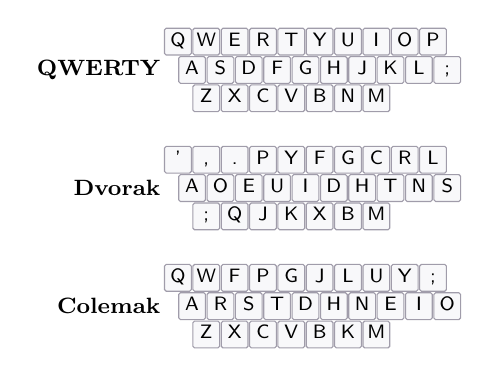
\begin{tikzpicture}
% Three keyboards stacked. Same 30 physical key positions; each layout
% reassigns the letters at those positions. Visual comparison highlights
% how a keymap is a re-binding of an unchanged physical substrate.
% Three keyboards stacked. Punctuation chars are wrapped in {} so
% TikZ's \foreach parser doesn't treat them as separators.
\foreach \layoutY/\name in {3.0/QWERTY, 1.5/Dvorak, 0.0/Colemak} {
 \node[anchor=east, font=\footnotesize\bfseries] at (-0.1, \layoutY+0.36) {\name};
}
% QWERTY rows
\foreach \l [count=\i] in {Q,W,E,R,T,Y,U,I,O,P}
 \node[kcap] at ({(\i-1)*0.36}, 3.72) {\strut\l};
\foreach \l [count=\i] in {A,S,D,F,G,H,J,K,L,{;}}
 \node[kcap] at ({(\i-1)*0.36+0.18}, 3.36) {\strut\l};
\foreach \l [count=\i] in {Z,X,C,V,B,N,M}
 \node[kcap] at ({(\i-1)*0.36+0.36}, 3.0) {\strut\l};
% Dvorak rows
\foreach \l [count=\i] in {{'},{,},{.},P,Y,F,G,C,R,L}
 \node[kcap] at ({(\i-1)*0.36}, 2.22) {\strut\l};
\foreach \l [count=\i] in {A,O,E,U,I,D,H,T,N,S}
 \node[kcap] at ({(\i-1)*0.36+0.18}, 1.86) {\strut\l};
\foreach \l [count=\i] in {{;},Q,J,K,X,B,M}
 \node[kcap] at ({(\i-1)*0.36+0.36}, 1.5) {\strut\l};
% Colemak rows
\foreach \l [count=\i] in {Q,W,F,P,G,J,L,U,Y,{;}}
 \node[kcap] at ({(\i-1)*0.36}, 0.72) {\strut\l};
\foreach \l [count=\i] in {A,R,S,T,D,H,N,E,I,O}
 \node[kcap] at ({(\i-1)*0.36+0.18}, 0.36) {\strut\l};
\foreach \l [count=\i] in {Z,X,C,V,B,K,M}
 \node[kcap] at ({(\i-1)*0.36+0.36}, 0) {\strut\l};
\end{tikzpicture}}
\caption{同一物理基底之上的三套打字键位映射。每一种布局都是把相同的按键位置重新绑定到另一组字母。QWERTY（Sholes 1873，从未申请专利）、Dvorak（Dvorak 与 Dealey 1936，US 2{,}040{,}248）、Colemak（Coleman 2006，公有领域）。2010 年之后的分叉生态延续了这一脉络。}
\label{fig:typing-layouts}
\end{figure}

\section{谱系二：乐器布局}
\label{sec:lineage2}

乐器布局走过一段平行的历史。Paul von Jankó 的六排同构钢琴键盘~\citep{janko1882}曾得到 Liszt 与 Rubinstein 的背书，由 Decker、Blüthner 与 Bösendorfer 制造，并在纽约的一所 Janko 音乐学院里教授。按照采纳所需的每一项社会先决条件，它都本应取代标准钢琴键盘。它没有。已知存世的 Janko 钢琴不足十架。Janko 案例是键位映射作为社会软件这一论证的反面极点：传播的每一项条件都已满足，传播却仍然失败。无论社会软件契约究竟是什么，它都不止是背书、制造商与音乐学院之和。

R.\ H.\ M.\ Bosanquet 的广义键盘~\citep{bosanquet1875generalized}是一台 53 平均律（53-EDO）的等音簧风琴，以及一台 1875 年以 48 音裂谬律与四分之一逗号中庸律调音的管风琴，于 1876 年在 South Kensington Museum 展示。它是基本上每一台现代同构控制器的先祖。Kaspar Wicki 于 1896 年为班多钮琴取得一项同构音位布局的专利~\citep{wicki1896}；六角手风琴演奏者 Brian Hayden 于 1986 年独立地重新发明并重新申请了基本相同的布局。相隔九十年的两度发明本身就是一项论证：这一布局具有\emph{发现}的性质，是那类因音乐底层结构使其有用而反复出现的对象，而非一件独特的文化器物。

\begin{figure}[t]
\centering
\resizebox{0.88\columnwidth}{!}{%
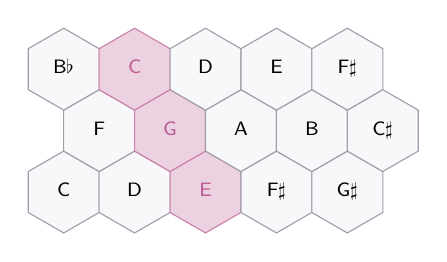
\begin{tikzpicture}
% Compact Wicki-Hayden-style hex schematic. Same-row neighbors
% differ by a whole tone; up-and-right neighbors differ by a P4.
% C major triad (C-E-G) highlighted; the same shape transposes to
% any key by translation across the surface ("isomorphism" claim).
% Hexes are EXPLICIT PATHS, not regular-polygon nodes — TikZ node
% sizing breaks the lattice. Pointy-top hexagon, circumradius R:
% width = sqrt(3)R, height = 2R. Tessellation: horizontal pitch =
% sqrt(3)R, row step = 1.5R, odd-row offset = sqrt(3)R/2.
\def\R{0.52}
\def\hexn#1#2#3{\begin{scope}[shift={(#1,#2)}]
 \draw[keystroke, fill=keyfill]
  (30:\R) -- (90:\R) -- (150:\R) -- (210:\R) -- (270:\R) -- (330:\R) -- cycle;
 \node[font=\scriptsize\sffamily, inner sep=0pt] at (0,0) {\strut#3};
\end{scope}}
\def\hexm#1#2#3{\begin{scope}[shift={(#1,#2)}]
 \draw[keymapped!70, fill=keymapped!25]
  (30:\R) -- (90:\R) -- (150:\R) -- (210:\R) -- (270:\R) -- (330:\R) -- cycle;
 \node[font=\scriptsize\sffamily, text=keymapped!90, inner sep=0pt] at (0,0) {\strut#3};
\end{scope}}
\def\hp{0.9006}  % horizontal pitch (sqrt(3) * R)
\def\vp{0.78}   % vertical pitch (1.5 * R)
\def\offx{0.4503} % horizontal offset for alternate rows (hp / 2)
% Row 0 (bottom)
\hexn{0}{0}{C}
\hexn{\hp}{0}{D}
\hexm{2*\hp}{0}{E}
\hexn{3*\hp}{0}{F$\sharp$}
\hexn{4*\hp}{0}{G$\sharp$}
% Row 1 (middle, offset)
\hexn{\offx}{\vp}{F}
\hexm{\offx + \hp}{\vp}{G}
\hexn{\offx + 2*\hp}{\vp}{A}
\hexn{\offx + 3*\hp}{\vp}{B}
\hexn{\offx + 4*\hp}{\vp}{C$\sharp$}
% Row 2 (top)
\hexn{0}{2*\vp}{B$\flat$}
\hexm{\hp}{2*\vp}{C}
\hexn{2*\hp}{2*\vp}{D}
\hexn{3*\hp}{2*\vp}{E}
\hexn{4*\hp}{2*\vp}{F$\sharp$}
\end{tikzpicture}}
\caption{Wicki--Hayden 六边形布局（Wicki 1896 / Hayden 1986）。同排相邻者相差一个全音；右上方相邻者相差一个纯四度。C 大三和弦（$C\,E\,G$）被高亮：该和弦是界面上一个固定的三格形状，而平移这一形状就把和弦移调到任意调。“移调即平移”是同构键盘的核心主张，也是标准钢琴白黑键不对称所牺牲掉的性质。}
\label{fig:wicki}
\end{figure}

\begin{figure*}[t]
\centering
% Interval-signature bars (full text width). Each bar reads left to
% right as the sequence of intervals the instrument's layout steps
% through; every block is one interval, its WIDTH = its size in
% semitones and its COLOR fixed by the legend. A regular instrument
% is a row of equal blocks; an asymmetric one has a visible odd block.
\begingroup
\definecolor{iv1}{HTML}{E2574C}% m2 (1 semitone)
\definecolor{iv2}{HTML}{EE9B3A}% M2 (2)
\definecolor{iv3}{HTML}{D1A52A}% m3 (3) — darkened so white slice text reads
\definecolor{iv4}{HTML}{4FAE54}% M3 (4)
\definecolor{iv5}{HTML}{3A86D6}% P4 (5)
\definecolor{iv7}{HTML}{8A5CF6}% P5 (7)
\resizebox{\textwidth}{!}{%
\begin{tikzpicture}
\def\rad{1.55}
% \pie{xshift}{name}{deg-per-semitone}{ semitones/color/label, ... }
% Slices sweep clockwise from 12 o'clock; angle = semitones. A regular
% instrument is an even wheel; an asymmetric one has a visibly odd slice.
% list fields: semitones / fill / interval-label / note-label.
% The note sits INSIDE the slice (the actual open string, scale degree,
% or valve number); the interval name sits just outside the rim.
\def\pie#1#2#3#4{\begin{scope}[shift={(#1,0)}]
 \xdef\angA{90}
 \foreach \s/\c/\lab/\nt in {#4}{
  \pgfmathsetmacro\angB{\angA-\s*#3}
  \filldraw[fill=\c, draw=\c!55!black, line width=0.6pt]
   (0,0) -- (\angA:\rad) arc[start angle=\angA, end angle=\angB, radius=\rad] -- cycle;
  \pgfmathsetmacro\angM{(\angA+\angB)/2}
  \node[font=\large\sffamily\bfseries, text=white] at (\angM:{0.58*\rad}) {\nt};
  \node[font=\small\sffamily, text=acdark] at (\angM:{\rad+0.32}) {\lab};
  \xdef\angA{\angB}
 }
 \node[font=\normalsize\sffamily\bfseries, text=acdark] at (0,{-\rad-1.08}) {#2};
\end{scope}}
% --- legend ---
\begin{scope}[shift={(-0.4,3.15)}]
 \node[font=\small\sffamily\bfseries, text=acdark, anchor=west] at (0,0.28) {音程 \;（扇区角度 $\propto$ 半音数）：};
 \def\lg#1#2#3{\draw[fill=#2, draw=#2!55!black, rounded corners=2pt] (#1,0.0) rectangle (#1+0.56,0.56);
  \node[font=\small\sffamily, text=acdark, anchor=west] at (#1+0.66,0.28) {#3};}
 \lg{7.7}{iv1}{m2}\lg{9.1}{iv2}{M2}\lg{10.5}{iv3}{m3}\lg{11.9}{iv4}{M3}\lg{13.3}{iv5}{P4}\lg{14.7}{iv7}{P5}
\end{scope}
% --- four wheels in a row ---
\pie{0}{Guitar \textperiodcentered\ EADGBE}{15}{5/iv5/P4/E, 5/iv5/P4/A, 5/iv5/P4/D, 4/iv4/M3/G, 5/iv5/P4/B}
% emphasize the guitar's lone M3 wedge (starts -135, spans 60 deg)
\draw[keymapped, line width=1.5pt]
 (0,0) -- (-135:\rad) arc[start angle=-135, end angle=-195, radius=\rad] -- cycle;
\pie{4.7}{Violin \textperiodcentered\ GDAE}{17.142857}{7/iv7/P5/G, 7/iv7/P5/D, 7/iv7/P5/A}
\pie{9.4}{Trumpet \textperiodcentered\ 3 valves}{60}{2/iv2/M2/1, 1/iv1/m2/2, 3/iv3/m3/3}
\pie{14.1}{Ocarina \textperiodcentered\ diatonic}{30}{2/iv2/M2/C, 2/iv2/M2/D, 1/iv1/m2/E, 2/iv2/M2/F, 2/iv2/M2/G, 2/iv2/M2/A, 1/iv1/m2/B}
\end{tikzpicture}}
\endgroup
\caption{四种不对称音高界面，读作\emph{音程轮}。每个轮顺时针扫过其布局所由构成的音程；每一扇区都是一个音程，其角度由其半音数大小设定，其颜色由图例固定。规则的乐器是一只均匀的轮；不对称的乐器则带有一个显眼的奇异扇区。吉他 EADGBE 是一圈纯四度，被 G 与 B 之间的大三度打破一次（已勾边）——正是这一不规则让标准和弦形状落在手下，民谣、布鲁斯、爵士与摇滚吉他也都是依此谱写的。小提琴是三个完全相同的纯五度：一只完美均匀的轮，可每根空弦各为一个不同的绝对音高。小号的三个活塞分别把音高降低两个、一个、三个半音——按设计各不相同，故其组合可达每一个半音级。陶笛是全音阶自身的轮，五个长步之间夹着两个短步。标准钢琴属于同一家族：那张全音阶命名键位映射体现在众多界面上，每一个都带有自己的不对称。}
\label{fig:asymmetric-instruments}
\end{figure*}

这些界面各自承载着自己的谱系。三活塞小号（Stölzel 与 Blühmel，约 1814 年）在一个世纪的自然小号实践之后标准化，其维也纳式与转阀式变体各自构成自身的音高之上的键位映射。陶笛从中美洲的器皿笛一路走到 Giuseppe Donati 于 1853 年在 Budrio 的标准化，那里不对称的指孔布置使得这套 10 孔图样得以教授。吉他的 EADGBE 调音于 1700 年代从琉特琴调音中结晶而成：B 弦的不规则打破了原本统一的四度，好让开放和弦形状落在手下，而整部民谣、布鲁斯、爵士与摇滚吉他的文献都是依着这一个不规则音程谱写的。小提琴严格的纯五度（G\,D\,A\,E）锚定了管弦乐曲目据以写就的、以五度为基础的弦乐声部惯例。在每一种情形里，不对称都不是音乐所容忍的缺陷，而是音乐据以谱写的一份继承——它决定了初学者最先学什么，一段练习曲长什么样，什么记法得以迁移。标准钢琴键盘坐落于这一传统之内，而非其上；那些同构的替代方案所提议的，比它们有时所承认的更为激进，那就是消解这张把所有这些乐器家族彼此相连的音高命名键位映射。

对 Jankó 失败——以及更广泛而言 Wicki--Hayden／六边形栅格家族之边缘地位——的标准解读，是按 David--Liebowitz 模型而来的路径依赖：钢琴仅凭锁定而延续。还有一种更艰难的解读。标准钢琴键盘的白黑不对称是一张半音圈的地标图——演奏者知道 $C$ 在哪，是因为它坐落在两个黑键之左——把绝对音高位置从记忆卸载给眼与手。剥去这种不对称，被卸载的信息便无处落脚：移调成了平移，但绝对位置成了回忆。四个世纪的曲目已把这种不对称吸收进\emph{调性格}——$F^\sharp$ 大调的指法不同于 $C$ 大调，而音乐正是依着这种差异写就的——故而移除这桩“历史的偶然”，会抹平文献据以谱写的一条意义之轴。这并不那么消解路径依赖的叙事，而是从另一侧沿着它切开：钢琴是路径依赖的，\emph{并且}这条路径已产出一件并不严格等价于其替代方案的对象。更深的一步是把西方调性体系本身当作一份键位映射：七字母全音阶命名 $C\,D\,E\,F\,G\,A\,B$ 已然是一份覆盖音高空间的社会软件契约，写进了理论、教学法与每一个调号。钢琴的白键是这份键位映射的物理实现；黑键则是记法早已用 $\sharp$ 与 $\flat$ 命名的变化音。标准钢琴因此一身二任——既是物理界面又是记法编码——而同构的替代方案提议消解后者以优化前者。这一论证被限定在以全音阶字母命名音高的十二平均律曲目之内；在其之外——19、22、31、53-EDO 的异律音乐，Maqam 以及别的带有不同音高命名键位映射的调性体系——钢琴是主动的阻碍，而从 Bosanquet 到 Lumatone 的同构脉络拥有一项强有力、扎根于曲目的主张。在那一范围之内，\texttt{notepat.com}（\textsection\ref{sec:notepat}）所保全的正是同一张音高命名键位映射，将其承载到 QWERTY 的字母键帽之上，按下字母 \texttt{C} 便弹奏音符 $C$。Jankó 消解命名键位映射以优化物理界面，半音阶梯式 DAW 约定则\emph{两者皆}消解（\textsection\ref{sec:daw}），而 \texttt{notepat.com} 保持命名契约不变，只重提 Sholes 在 1873 年的技工们所问的那个问题：什么样的物理界面应当把它向前承载。

其当代后裔是商业产品：C-Thru AXiS-49（2008）~\citep{cthru2008axis49}、Jim Plamondon 的 Thummer~\citep{plamondon2003thummer}、Roger Linn LinnStrument、ROLI Seaboard、Lumatone 六边形栅格，以及 Lippold Haken 的 Continuum Fingerboard~\citep{haken1998indiscrete}。Andrew Milne、William Sethares 与 James Plamondon 关于同构控制器与调音连续统的论文~\citep{milne2007isomorphic,milne2008tuning}提供了理论基础。从键位映射作为社会软件的视角看，引人注目的是这些乐器\emph{出厂即可配置}：布局是一个由用户上传的显式对象，而异律社群以文件的形式分享布局。Lumatone 尤其把键位映射当作分发的单位。乐器是基底；键位映射才是使其成为乐器的那件器物。

\section{半音阶梯，或曰 AWSED：无所有权的趋同}
\label{sec:daw}

键位映射作为社会软件这一论证最有力的当代案例，是每一款主流数字音频工作站所共享的、事实上的半音阶梯式 QWERTY 钢琴键位映射。Ableton Live、Logic Pro、GarageBand 与 FL Studio 全都默认附带同一套约定~\citep{ableton_musical_typing,apple_logic_musicaltyping,imageline_typing_piano}。这套约定的形状是：取 QWERTY 键盘下方三排；把其中一排当作从 C 上行的半音阶白键；把其上一排当作黑键，置于钢琴上黑键本会落下的空隙处。Ableton、Logic 与 GarageBand 用 \keys{A,S,D,F,G,H,J,K}（主键行）作白键 $C\,D\,E\,F\,G\,A\,B\,C$，用 \keys{W,E,T,Y,U}（上方一排）作黑键 $C^\sharp\,D^\sharp\,F^\sharp\,G^\sharp\,A^\sharp$。FL Studio 用底行 \keys{Z,X,C,V,B,N,M} 作低八度的白键，并用同样的上方一排图样作黑键。原则完全相同。具体的排位指派差了一排。

这套约定已传播三十年而无名。我在此为本应研究它的那个领域命名它：把前五个半音音级所落的按键——$C$ 在 \key{A}，$C^\sharp$ 在 \key{W}，$D$ 在 \key{S}，$D^\sharp$ 在 \key{E}，$E$ 在 \key{D}——按音高顺序读出，它们拼成 \textbf{AWSED}。\emph{此后即称 AWSED 布局}（主键行变体；FL Studio 变体是它的底行移位）。这个名字之所以选来与下文讨论的 PC 游戏移动约定 WASD 押韵，是因为两者在结构上是同一对象——一份无人设计、人人附带、无所有权、无规范、跨应用的输入键位映射——而这押韵本身就是论证。WASD 被它的社群命名、教授并奉为经典；AWSED 却连名字都从未有过，而这恰恰是它逃过研究的原因。一件没有名字的东西难以被看见，更难以被批评，也不可能被引用。为它命名是第一步。

没有人设计了这套约定。没有规范界定它。没有治理机构，没有维护者，没有资助机制。这套约定得以存在，是因为这四种实现彼此一致，而这四种实现彼此一致，是因为这套约定早已存在于先于现代 DAW 的 1990 年代追踪器软件（FastTracker、Renoise、Impulse Tracker）之中，也是因为凡是学过一款 DAW 的用户都预期下一款行为相同。为一款 DAW 写的教程文档，或多或少能迁移到另一款。这就是最纯粹形态的\emph{社会软件契约}：一件透过教学与预期传播、毫无中央权威的可版本化虚拟对象。

\begin{figure}[t]
\centering
\resizebox{\columnwidth}{!}{%
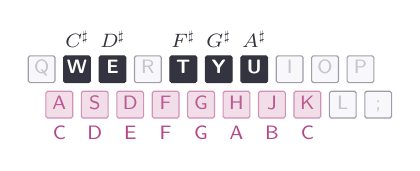
\begin{tikzpicture}
% Upper QWERTY row (sharps in DAW chromatic-staircase). Only 5 keys
% are mapped (W E T Y U); R and I sit in the gaps with no note.
\foreach \l/\note/\mapped [count=\i] in {%
 Q/{}/0, W/$C^\sharp$/1, E/$D^\sharp$/1, R/{}/0, T/$F^\sharp$/1,
 Y/$G^\sharp$/1, U/$A^\sharp$/1, I/{}/0, O/{}/0, P/{}/0%
}{
 \ifnum\mapped=1
  \node[kcap sharp] (k\i) at ({(\i-1)*0.45}, 1.8) {\strut\l};
  \node[font=\scriptsize\sffamily, text=keysharp, anchor=south, inner sep=1pt]
   at ({(\i-1)*0.45}, 2.03) {\note};
 \else
  \node[kcap, text=keystroke!60] (k\i) at ({(\i-1)*0.45}, 1.8) {\strut\l};
 \fi
}
% Home row (whites). 8 of 10 keys mapped (A through K = C..C).
\foreach \l/\note/\mapped [count=\i] in {%
 A/C/1, S/D/1, D/E/1, F/F/1, G/G/1, H/A/1, J/B/1, K/C/1, L/{}/0, {;}/{}/0%
}{
 \ifnum\mapped=1
  \node[kcap mapped] at ({(\i-1)*0.45+0.225}, 1.35) {\strut\l};
  \node[font=\scriptsize\sffamily, text=keymapped, anchor=north, inner sep=1pt]
   at ({(\i-1)*0.45+0.225}, 1.12) {\note};
 \else
  \node[kcap, text=keystroke!60] at ({(\i-1)*0.45+0.225}, 1.35) {\strut\l};
 \fi
}
\end{tikzpicture}}
\caption{AWSED 布局——DAW 半音阶梯式 QWERTY 钢琴键位映射（Ableton、Logic、GarageBand 变体）。主键行 \texttt{A~S~D~F~G~H~J~K} 弹奏 $C$ 到 $C$ 的白键；其上一排把升号置于钢琴黑键本会落下的空隙处（$C^\sharp\,D^\sharp$，然后在 \texttt{R} 处有一个空隙，$F^\sharp\,G^\sharp\,A^\sharp$，再是空隙）。这个名字来自前五个半音音级 $C\,C^\sharp\,D\,D^\sharp\,E$，它们落在 \key{A}\,\key{W}\,\key{S}\,\key{E}\,\key{D} 上。每个键帽上的 QWERTY 字母与它所产生的音名毫无关系。}
\label{fig:daw-staircase}
\end{figure}

我还将论证，它的设计也很糟糕。AWSED 布局有三处结构性弱点。\textbf{其一}，每个键上的 QWERTY 字母与它所产生的音名毫无关系。\key{A} 弹奏 C；\key{S} 弹奏 D；\key{D} 弹奏 E（图~\ref{fig:daw-staircase}）。学过西方七音音阶的用户无法凭这一知识在该键位映射上获得任何抓手。\textbf{其二}，它只提供单个八度（$C$ 到 $C$），却把这一个八度横铺过整条主键行，从 \key{A} 一直到 \key{K}——正是\emph{双手}都搁着的整片宽度。它既不是紧凑的单手八度，也不是高产的双手音域：它耗用两只手的键盘只产出一个八度，便就此打住。其宽度铺得仿佛是给两只手的，音域却按一只手来定。\textbf{其三}，没有教程便无法读懂这份键位映射：没有助记符，物理键上没印任何图示，也无从根据第一性原理推导出该映射。需要手册的键位映射，就是失去了社会软件性格的键位映射。

为它命名并非闲笔。它天然的对照物是 WASD，PC 游戏中的移动约定——而这近乎易位构词的关系与其说是巧合，不如说是一项诊断。WASD 与 AWSED 有着相同的结构形状——一份无人拥有、无规范、跨应用的用户输入约定——但有着不同的传播史。在 WASD 之前，PC 游戏默认用方向键（Wolfenstein 3D、Doom、直到 1997 年的 Quake 系列）~\citep{wikipedia_arrow_keys}；中间的试验包括 System Shock 的 ASDX（1994）与 Descent 的 AZ+QE。竞技 Quake 玩家 Dennis “Thresh” Fong 透过其自费出版的配置指南~\citep{thresh_quake_bible}推广了 WASD 布局，并于 1997 年赢得了首届全国性 Quake 锦标赛。Valve 的 Half-Life 于 1998 年默认附带 WASD，到 2000 年代初这套约定已饱和 PC 游戏~\citep{fenlon2016wasd}。WASD 得以延续，原因正是 DAW 半音阶梯所不具备的：它确实比官方默认更好。它把右手解放给鼠标，紧邻 Shift / Space / Ctrl / Tab，并利用了 QWERTY 键盘上主键行的手指位置。其结构性教训是，传播是社会中介\emph{与}适应度二者的函数：WASD 得以传播，是因为 Fong 的教学触及了玩家，\emph{并且}这份映射凭实力取胜。半音阶梯仅凭教学传播，尽管实力恰恰相反。两个案例都坐落于同一范畴——跨应用治理用户输入的无主约定。它们表明，这一范畴大到足以横跨良设计与劣设计、用户验证与因惯性而继承两端。

\section{Notepat.com：为自己命名的音符}
\label{sec:notepat}

针对这位既有者，\texttt{notepat.com} 提议了一份不同的键位映射（图~\ref{fig:notepat-keymap}）。其设计原则只有一条：\emph{为自己命名的音符}。QWERTY 字母 \key{C} 弹奏 C。QWERTY 字母 \key{D} 弹奏 D。西方音阶的七个本位音——$C\,D\,E\,F\,G\,A\,B$——弹奏其字母所命名的音符。上方八度继续按字母排列：\keys{H,I,J,K,L,M,N} 对应 $C_5\,D_5\,E_5\,F_5\,G_5\,A_5\,B_5$。升号在 QWERTY 字母允许之处落在其本位音上方一排，类比于钢琴黑键：\keys{V,S,W,R,Q} 对应 $C^\sharp\,D^\sharp\,F^\sharp\,G^\sharp\,A^\sharp$。低八度落在左手之下；高八度落在右手之下。

这份键位映射逐一逆转了 AWSED 的三处弱点。\textbf{其一}，每个键上的字母\emph{就是}音名。任何懂西方音阶的人都已经懂这份键位映射。\textbf{其二}，它高产地耗用那片双手宽度：左手弹低八度，右手在高八度上镜像它，于是 AWSED 用以产出单个八度的同一片跨度在这里产出两个。\textbf{其三}，这份键位映射自带文档：图~\ref{fig:notepat-keymap}中的图示，任何能拼出“CDEFGAB”的人都能凭记忆复现。

有三件事使 \texttt{notepat.com} 在本文的诸键位映射中显得不寻常：它有一个名字——大多数（如 AWSED，\textsection\ref{sec:daw}）从未有过——它的音符为自己命名，于是这份键位映射指涉自身，而且它已经运行在许多种实现之中。\texttt{notepat.com} 的贡献并不在于实现。其实现按设计是朴素的：几百行 JavaScript，把键盘事件路由到一套音频合成 API。贡献在于键位映射。它呈现于五种实现之中——\texttt{notepat.com} 上的网页作品、AC Native OS 的裸机移植、MenuBand 这款 macOS 菜单栏应用、Ableton（Max for Live）插件，以及 \texttt{babypat}——而键位映射是这一切之中唯一在全部实现里都完全相同的东西。这套音符命名记法迁移得比乐器本身还远：它在 \texttt{clock}（AC 的分布式音序器）中被复用，那里同样的单字母音高驱动着联网的播放。它就是那份 \texttt{notepat.com} 形状的社会软件契约。

将各实现并排比较的读者会注意到，有些键做着超出图~\ref{fig:notepat-keymap}中那张表的事。在 AC Native 与 MenuBand 上，按住 \texttt{Space} 会倒放最近几秒的实际音频输出。在网页作品与 AC Native 上，敲击一个音符时按住 \texttt{Shift}，会在松开时给那个声部一条长长的衰减尾巴；按住 \texttt{Enter} 会无限延持该声部，而 \texttt{Backspace} 清除每一个被延持的声部。在 MenuBand 与 AC Native 上，\texttt{Control}、\texttt{Alt} 以及二者并用，会把单次按键升格为一个大三、小三或挂留三和弦。这一切都不出现在键位映射图示中，而这一省略是有意的。这些绑定构成一个\emph{扩展演奏层}，而该层与音调映射之间的界线，正是社会软件契约本身的边界（表~\ref{tab:contract-line}）。

\begin{table}[t]
\footnotesize
\setlength{\tabcolsep}{3pt}
\renewcommand{\arraystretch}{1.05}
\centering
\caption{\texttt{notepat.com} 的诸绑定，在契约线处划分。线之上：音调映射，在所有实现里完全相同——社会软件对象。线之下：扩展演奏层，每一种底层都可自由有别。}
\label{tab:contract-line}
\begin{tabularx}{\columnwidth}{@{}>{\RaggedRight}p{0.30\columnwidth}>{\RaggedRight}X>{\RaggedRight\arraybackslash}p{0.21\columnwidth}@{}}
\toprule
\textbf{绑定} & \textbf{含义} & \textbf{何处} \\
\midrule
\multicolumn{3}{@{}l}{\emph{音调契约}} \\[0.1em]
\texttt{C D E F G A B} & 本位音 $C_4$--$B_4$，左手 & 全部 \\
\texttt{H I J K L M N} & 本位音 $C_5$--$B_5$，右手 & 全部 \\
\texttt{V S W R Q} & 升号，上方一排 & 全部 \\
\midrule
\multicolumn{3}{@{}l}{\emph{扩展演奏层}} \\[0.1em]
\texttt{Shift}（按住） & 延音：长衰减尾巴 & 网页、Native \\
\texttt{Enter}（按住） & 延持声部；\texttt{Backspace} 清除 & 网页、Native \\
\texttt{Space}（按住） & 倒放近期音频 & Native、MenuBand \\
\texttt{Ctrl}\,/\,\texttt{Alt}\,/\,二者 & 大三\,/\,小三\,/\,挂二和弦 & MenuBand、Native \\
\texttt{<}~\texttt{>} & 各手八度移位 & 网页 \\
\bottomrule
\end{tabularx}
\end{table}

表~\ref{tab:contract-line}的两半受不同规则支配。线之上，偏离即破坏：一个把 \texttt{C} 从音符 $C$ 重新映射开去的实现，将不是一个 \texttt{notepat.com} 移植，而是一件不同的乐器。线之下，偏离即惯用：每一种底层都生长出其躯体所允许的手势。裸机操作系统拥有整台机器，便能环形缓冲自身的音频输出并倒着播放；菜单栏应用骑在系统级事件捕获之上，便倚重修饰键和弦；网页作品栖身于浏览器标签页之内，便延音与延持。用户并不把这些差异体验为破坏，也没有哪个实现有义务承载另一个的手势。同样的两级结构在更老的案例里也可见：QWERTY 作为契约对媒体键或 \texttt{Fn} 层只字未提，它们随厂商自由变化，却没人把 ThinkPad 称作 QWERTY 的一个分叉；Vim 的核心动作是契约，而插件绑定是惯用。这暗示，一份键位映射并不是某个实现所附带的全部绑定的集合。它是其中这样一个子集：对其加以变更，社群会体验为对身份的违背——而判断某个绑定落在线的哪一侧，一项实用检验就是看记法表面（\textsection\ref{sec:notation}）是否承载它。\texttt{C D E F G A B} 作为文本迁移；“按住空格倒转时间”则是一种逐底层的手势，必须在每一次移植时经由示范重新教授。

这就是本文请读者去看见的那一步。主导的 DAW 半音阶梯式键位映射从未被\emph{选择}——它是从追踪器软件\emph{继承}而来，凭用户预期而延续，并经跨应用约定而锁定。\texttt{notepat.com} 表明这道缝隙是敞开的：一个有意设计的替代方案，可以由单个开发者用几百行代码写就，在一年之内跨多种实现交付，并作为一份竞争性的社会软件契约献给更广的社群。这其中的政治赌注在任一单例里都很小，在总体上却很大：\emph{这道缝隙处处敞开}。

\section{记法：论说的表面}
\label{sec:notation}

至此为止的论证一直把键位映射当作一张表。但键位映射不只是一张表。它还有一种\emph{记法}——一种文本形式，键位映射的用法正是在其中被阅读、书写、教授、引用与争论。记法是键位映射论说的表面。我还将论证，它是键位映射中真正会迁移的那一半。记法可移植的键位映射作为文本传播；记法笨拙或缺失的键位映射只作为肌肉记忆传播。因此记法的品质是键位映射一项可供设计的属性，而非派生的器物。一个只交付绑定表的设计者，只交付了这件对象的一半。

典范案例是 Vim。Vim 底层的键位映射是一张把击键映射到编辑器命令的表：\texttt{d} 发起一个删除算子，\texttt{i} 一个内文本对象，\texttt{w} 一个词动作。然而在 Vim 论说中迁移的并不是这张表。迁移的是一种\emph{记法}：\texttt{dd}、\texttt{ciw}、\texttt{gg}、\texttt{:wq}、\texttt{<C-w>}（图~\ref{fig:vim-modes}）。教程、博文、README 文件、vimtutor，以及长盛不衰的 vim 对 emacs 之争，全都以这种记法进行。这种记法可移植到甚至完全在 Vim 之外存活：\emph{vim 模式}出现在 Visual Studio Code、在 JupyterLab、在通过 \texttt{set -o vi} 的各种 shell、在 macOS Cocoa 文本框、在通过 Vimium 的浏览器里。被移植的是记法。运行时是偶然的。

\begin{figure}[t]
\centering
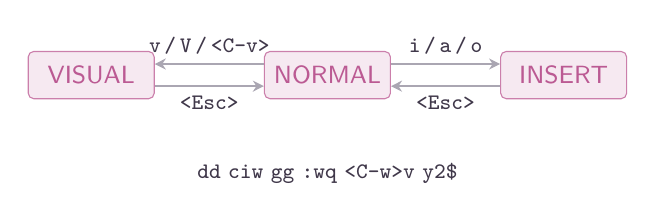
\begin{tikzpicture}[
 modebox/.style={draw=keymapped!70, fill=keymapped!12,
          rounded corners=2pt, minimum width=1.6cm,
          minimum height=0.6cm, font=\small\sffamily,
          text=keymapped!90, inner sep=2pt},
 arrow/.style={-{Stealth[length=4pt,width=4pt]}, draw=keystroke!90,
         line width=0.5pt},
 cmd/.style={font=\footnotesize\ttfamily, text=acdark}
]
% Three Vim modes wired by their command-notation transitions.
\node[modebox] (normal) at (0, 0) {NORMAL};
\node[modebox] (insert) at (3.0, 0) {INSERT};
\node[modebox] (visual) at (-3.0, 0) {VISUAL};
\draw[arrow] ([yshift=4pt]normal.east) -- node[above, cmd] {\texttt{i}\,/\,\texttt{a}\,/\,\texttt{o}} ([yshift=4pt]insert.west);
\draw[arrow] ([yshift=-4pt]insert.west) -- node[below, cmd] {\texttt{<Esc>}} ([yshift=-4pt]normal.east);
\draw[arrow] ([yshift=4pt]normal.west) -- node[above, cmd] {\texttt{v}\,/\,\texttt{V}\,/\,\texttt{<C-v>}} ([yshift=4pt]visual.east);
\draw[arrow] ([yshift=-4pt]visual.east) -- node[below, cmd] {\texttt{<Esc>}} ([yshift=-4pt]normal.west);
% A row of canonical commands underneath
\node[font=\footnotesize\ttfamily, text=acdark, anchor=north] at (0, -1.0)
 {\texttt{dd}\,\,\texttt{ciw}\,\,\texttt{gg}\,\,\texttt{:wq}\,\,\texttt{<C-w>v}\,\,\texttt{y2}\$};
\end{tikzpicture}
\caption{Vim 的模式化键位映射及其迁移的记法。各模式（NORMAL、INSERT、VISUAL）由带标注的击键转换相连；常用命令（\texttt{dd} 删除行、\texttt{ciw} 改内词、\texttt{gg} 至顶、\texttt{:wq} 写入并退出等）是这份键位映射的论说货币。这套记法可移植到已被在 VS~Code、JupyterLab、Vimium、macOS Cocoa 文本系统与 \texttt{set -o vi} 中重新实现。}
\label{fig:vim-modes}
\end{figure}

DAW 半音阶梯是反面案例。它没有可移植的记法。要写下一段在 Ableton 音乐打字上弹奏的旋律，只能退回到事件序列的散文——“按 \key{A}，再按 \key{S}，再按 \key{D}”——这描述的是输入而非音乐。相比之下，Singmaster 魔方记法~\citep{singmaster1981notes}（图~\ref{fig:singmaster}）让 \texttt{R U R' U' R U2 R'} 把一套魔方算法在玩魔方者之间完整迁移；或纳什维尔数字体系~\citep{matthews1984nashville,williams1988nashville}，让“1--4--5”把一段和弦进行在录音室乐手之间迁移；或 Plover 速记理论~\citep{knight2010plover}，让和弦记法把速记图样透过社群编纂的词典迁移。DAW 阶梯没有这样的把手。它的键只能凭物理位置寻址。因此这份键位映射存在于肌肉记忆里，鲜少落于纸面——这恰恰是它尽管用户群可能更大、论说存在感却低于 Vim 的原因。

\begin{figure}[t]
\centering
\resizebox{0.62\columnwidth}{!}{%
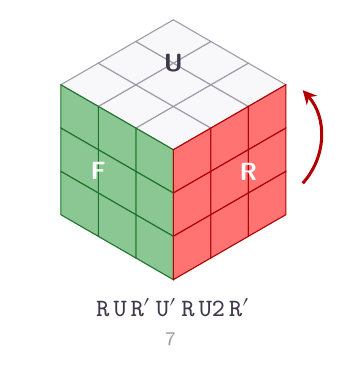
\begin{tikzpicture}
% Symmetric bounding box around the cube body (x=0) so \centering
% lands it centered --- the quarter-turn arrow otherwise extends the
% natural box rightward and pulls the cube off-center.
\useasboundingbox (-1.85,-2.55) rectangle (1.85,1.55);
% Isometric Rubik's cube, three visible faces: U (top), F (front-
% left), R (right). Faces are explicit-path parallelogram grids built
% from iso axes er=(0.866,0.5)s (right-up), el=(-0.866,0.5)s
% (left-up), ed=(0,-1)s (down), all meeting at the shared front-top
% vertex at the origin. The R face is tinted with a quarter-turn
% arrow: the diagram shows the first move of the algorithm below.
\def\s{0.55}
% Top face U: cells spanned by er and el
\foreach \i in {0,1,2} \foreach \j in {0,1,2}
 \draw[keystroke, fill=keyfill]
  ({0.866*\s*(\i-\j)}, {0.5*\s*(\i+\j)})
  -- ++({0.866*\s}, {0.5*\s})
  -- ++({-0.866*\s}, {0.5*\s})
  -- ++({-0.866*\s}, {-0.5*\s}) -- cycle;
% Front-left face F: cells spanned by el and ed — green stickers
\foreach \i in {0,1,2} \foreach \j in {0,1,2}
 \draw[acgreen!75!black, fill=acgreen!55]
  ({-0.866*\s*\i}, {0.5*\s*\i - \s*\j})
  -- ++({-0.866*\s}, {0.5*\s})
  -- ++(0, {-\s})
  -- ++({0.866*\s}, {-0.5*\s}) -- cycle;
% Right face R: cells spanned by er and ed — red stickers (mid-turn)
\foreach \i in {0,1,2} \foreach \j in {0,1,2}
 \draw[red!70!black, fill=red!55]
  ({0.866*\s*\i}, {0.5*\s*\i - \s*\j})
  -- ++({0.866*\s}, {0.5*\s})
  -- ++(0, {-\s})
  -- ++({-0.866*\s}, {-0.5*\s}) -- cycle;
% Face labels at face centers — standard sticker scheme:
% white up, green front, red right.
\node[font=\small\sffamily\bfseries, text=acdark]
 at (0, {1.5*\s + 0.5*\s}) {U};
\node[font=\small\sffamily\bfseries, text=white]
 at ({-0.866*\s*1.5 - 0.433*\s}, {0.75*\s - 1.5*\s + 0.25*\s}) {F};
\node[font=\small\sffamily\bfseries, text=white]
 at ({0.866*\s*1.5 + 0.433*\s}, {0.75*\s - 1.5*\s + 0.25*\s}) {R};
% Quarter-turn arrow for R: curved arrow hugging the right face's
% outer edge, pointing upward (clockwise as seen from the right).
\draw[-{Stealth[length=5pt,width=5pt]}, line width=1.1pt, red!70!black]
 ({0.866*\s*3.45}, {0.5*\s*3.45 - 2.5*\s})
 to[bend right=42]
 ({0.866*\s*3.45}, {0.5*\s*3.45 - 0.35*\s});
% Notation row underneath
\node[font=\small\ttfamily, anchor=north, text=acdark]
 at (0, {-3.2*\s}) {R\,U\,R$'$\,U$'$\,R\,U2\,R$'$};
\node[font=\scriptsize\sffamily, anchor=north, text=keystroke]
 at (0, {-4.0*\s}) {一套 7 步算法};
\end{tikzpicture}}
\caption{Singmaster 的魔方记法~\citep{singmaster1981notes}。每个大写字母命名一个面（\textsf{U}p 上、\textsf{D}own 下、\textsf{L}eft 左、\textsf{R}ight 右、\textsf{F}ront 前、\textsf{B}ack 后）；裸字母是顺时针四分之一转，带撇字母（$\,'$）是逆时针四分之一转，数字 2 是半转。七记号串 \texttt{R U R$'$ U$'$ R U2 R$'$} 是一套完整算法，可在玩魔方者、GitHub 仓库与 YouTube 教程之间移植——键位映射—记法这一配对作为文本迁移。各面采用标准贴纸方案（白上、绿前、红右）；\textsf{R} 画作正处于四分之一转之中：算法的第一步。}
\label{fig:singmaster}
\end{figure}

\texttt{notepat.com} 的“音符为自己命名”设计有一个结构性副作用：一套学起来不费分文的记法。要写一段 notepat.com 序列，写下 \texttt{C D E F G A B} 即可——这同时也是标准乐谱记法。这套记法不是为 \texttt{notepat.com} 发明的；它是从既有的一种素养\emph{继承}来的。一位从未见过 notepat.com 键位映射的钢琴家能读懂一份 notepat.com 乐谱；反过来，一位学会该键位映射的 notepat.com 演奏者也同时在演练标准的音高字母素养。这就是一个良好设计的记法表面的样子：记法是如此轻易地从先验知识中可推导，以致学习记法不费分文。相比之下，Ableton 的半音阶梯会要求把一份 notepat 式的乐谱重新编码为 \texttt{A S D F G H J}——一套拴在单一键位映射上、别处毫无用处的私有记法。

关于键盘快捷键采纳的经验文献支持这一读法。Peres 等人发现，与其他快捷键用户共事，比单纯的计算机经验更能预测快捷键的使用~\citep{peres2004shortcut}。Lozhkina 等人延伸了这一结果：快捷键的发现渠道是人际的与视觉的~\citep{lozhkina2025discovery}。Wang 等人明确使用\emph{词汇}（vocabulary）一词来命名快捷键设计交给用户的东西~\citep{wang2020keymap}。本文的论证使这些发现更为锐利：社会中介并非身处其他用户之间所产生的一种泛泛效应；它是一种经由记法表面的特定传递。同事互相读对方的屏幕，看见 \texttt{:wq}，发问，学会。哪里没有可传递的记法，哪里就没有社会中介可供中介。同样的逻辑也解释了现场编码迷你记法的成功：Alex McLean 与 Geraint Wiggins 的 TidalCycles 图样语言~\citep{mclean2010tidal}，移植到 JavaScript 即为 Strudel~\citep{roos2023strudel}，以及 Olivia Jack 用于现场编码视觉的 Hydra 变换链~\citep{jack2018hydra}，连同用于民谣的 ABC 记法~\citep{walshaw_abc}。在每一种情形里，运行时都是偶然的——Haskell、JavaScript、WebGL、MIDI 播放器——但记法把这一实践带过了各种运行时、工作坊与数十年的岁月。

\textsection\ref{sec:corollaries}的推论目录，透过这一视角来读，几乎全然是一份记法目录。Singmaster、纳什维尔、ABC、IPA、Camelot、格斗游戏的小键盘记法、科学音高、北约拼读字母、编织缩写——每一个都是从某份键位映射（或输入映射）派生出的记法，它让底层实践得以作为文本迁移。键位映射—记法这一配对才是单位。键位映射提供可供性；记法提供传播表面。

这一结构性主张有一个更深的诊断。Walter Ong 关于口语性与文字性的区分~\citep{ong1982orality}，建立在 Havelock 对古希腊同一转变的论述之上~\citep{havelock1963preface}，把问题切得干净利落。\emph{口语}传统经由表演、人对人的传递与反复的近似而延续；它们没有正典文本，在各实例间略有变异，并因表演者持续表演而存活。\emph{文字}传统经由固定文本、权威版本与精确再现而延续；它们有规范、有正典、有参考实现。计算学术研究的标准框架全都是文字框架：一份开源许可证治理一段固定文本，一项协议治理一种固定线路格式，一种格式治理一种固定编码。DAW 半音阶梯是一份原生口语的键位映射——没有正典文本，只有四种凭表演而一致的实现。Vim 兼有口语基底（人是看着另一位开发者的屏幕学会这份键位映射的）与文字边缘（记法：\texttt{:wq}、\texttt{<C-w>}、\texttt{ciw}）。\texttt{notepat.com} 把文字一侧坍缩进音高字母记法这一现成素养：键位映射从一项更古老数世纪的文字实践中继承了它的书面形式。口语基底是键位映射；记法是文字的固定；后者成功之处，前者便获得一具会迁移的身体。口语—文字之轴正是键位映射何以根本逃脱开源／专有框架的诊断：标准框架是文字框架，而键位映射至少部分是口语的，学术与产业论说中同样缺乏文字固定，正是给了本文以推动力问题的那个症状。

同一口语—文字之轴解释了键位映射文献的一个特征：这种文献并不多。PC Gamer 那篇关于 WASD 的历史~\citep{fenlon2016wasd}，是一份关于掌控着数亿小时游戏时长的约定的、典范的大众媒体来源；对应的学术文献则基本是空白。这不是因为键位映射不重要。而是因为计算学术研究现有的装置——规范、RFC、源代码仓库——是为文字器物校准的，而键位映射部分是口语的。那篇并不存在的论文，恰恰就是本文论证理应存在的那一篇。

\section{推论目录}
\label{sec:corollaries}

键位映射只是一个大得多的属类的一个实例：\emph{经由社会契约而非二进制文件传播的可版本化虚拟对象}。表~\ref{tab:corollaries}编目了主要的物种。该目录并不穷尽。其用意是表明这一属类真实而庞大。

若干模式浮现出来。其一，这一属类横跨输入映射（QWERTY、Vim、WASD）、记法系统（Singmaster、纳什维尔、IPA）、范畴标签（手柄按键、CSS 颜色），以及社群作者化的首字母缩略（北约拼读字母；LGBTQ+ 缩略，其修订史——LGB $\rightarrow$ LGBT $\rightarrow$ LGBTQ $\rightarrow$ LGBTQIA $\rightarrow$ LGBTQIA2S+——本身就是一个无治理机构却版本化的过程，记录于各风格指南~\citep{glaad_reference_guide}）。统一它们的不是媒介而是\emph{角色}：每一个都是一张在人与机器之间、在实践共同体之间、或在竞争性实现之间的边界处被查阅的小型声明式表格。其二，具名发明者的模式高度多变。有些对象有单一具名发明者（Singmaster、Coleman、Davis）；另一些有趋同或匿名的起源（DAW 半音阶梯、格斗游戏小键盘记法）；又一些是社群版本化并带具名增补的（LGBTQ+ 缩略）；还有一些是在一段社群竞争之后由联盟结晶而成的（代数式国际象棋、BÉPO）。其三，传播机制几乎从不是二进制文件。它是教学、预期、引用或书面参考——一个文字共同体的装置。

这一范畴的边界值得清晰地划出。\textbf{开放格式}如 PNG 与 MP3 由规范与参考实现治理~\citep{sterne2012mp3}——更接近格式而非社会软件。\textbf{开放协议}如 HTTP 与 IRC 有 RFC 与管理机构——Galloway 的《Protocol》~\citep{galloway2004protocol}覆盖了这片地界。\textbf{民众分类法}（标签、话题标签）是内容分类而非作为对象的界面。\textbf{模因}会传播，但属于内容。键位映射与这一切都不同：\emph{一张中介输入／输出的小型声明式表格，没有治理机构，却依然表现得仿佛已被标准化}。

% X cells render as m{} (vertically centered, footnotesize) so single
% -line labels sit centered against wrapped propagation text. Defined
% OUT here (not inside \afterpage — a bare #1 breaks its tokenizer).
\renewcommand{\tabularxcolumn}[1]{>{\footnotesize}m{#1}}
% Full-width table as a proper float page ([p]): LaTeX fills the
% surrounding two-column text pages completely (no stranded column)
% and drops the table on its own float page. Label columns auto-size
% and never wrap; only the Propagation column flexes.
\begin{table*}[p]
\footnotesize
\setlength{\tabcolsep}{5pt}
\renewcommand{\arraystretch}{1.32}
\centering
\caption{选录的经由社会契约传播的可版本化虚拟对象。“发起者”列出存在具名发明者时的发明者；“\emph{conv.}”表示趋同或匿名的起源。每一行的二维码解析到该对象的正典之家——维基百科、项目自身的站点，或其治理规范。}
\label{tab:corollaries}
\arrayrulecolor{acgray!35}
\begin{tabularx}{\textwidth}{|@{\hspace{2.5pt}}c@{\hspace{2.5pt}}|>{\bfseries\color{acdark}}l|>{\color{acdark}}l|l|>{\RaggedRight\arraybackslash\color{acdark}}X|}
\hline
\cellcolor{acdark!75}{\color{white}\bfseries 扫描} &
\cellcolor{acpink!75}{\color{white}\bfseries 对象} &
\cellcolor{acpurple!75}{\color{white}\bfseries 发起者（年份）} &
\cellcolor{acblue!75}{\color{white}\bfseries 领域} &
\cellcolor{acgreen!75}{\color{white}\bfseries 传播} \\
\hline
\rowcolor{acblue!8} \qrc{qwerty} & QWERTY            & Sholes (1873)               & \dmn{acblue}{打字}  & 制造商采纳 $\rightarrow$ ISO/AFNOR $\rightarrow$ 操作系统布局文件 \\ \hline
\rowcolor{acblue!8} \qrc{dvorak} & Dvorak            & Dvorak \& Dealey (1936)          & \dmn{acblue}{打字}  & 美国专利 $\rightarrow$ 美国海军 $\rightarrow$ 用户自装的操作系统布局 \\ \hline
\rowcolor{acblue!8} \qrc{colemak} & Colemak           & Coleman (2006)               & \dmn{acblue}{打字}  & colemak.com + GitHub 分叉（Workman、Halmak、DH） \\ \hline
\rowcolor{acblue!8} \qrc{bepo} & BÉPO             & Community (2005)              & \dmn{acblue}{打字}  & 社群设计 $\rightarrow$ 2019 AFNOR 国家标准 \\ \hline
\rowcolor{acpink!8} \qrc{janko} & Janko            & Jankó (1882)                & \dmn{acpink}{音乐}   & \emph{传播失败}——反面案例研究 \\ \hline
\rowcolor{acpink!8} \qrc{wicki} & Wicki--Hayden         & Wicki (1896) / Hayden (1986)        & \dmn{acpink}{音乐}   & 六角手风琴社群 $\rightarrow$ 现代 MPE 控制器 \\ \hline
\rowcolor{acpink!8} \qrc{bosanquet} & Bosanquet          & Bosanquet (1875)              & \dmn{acpink}{音乐}   & 微分音社群 $\rightarrow$ Lumatone \\ \hline
\rowcolor{acpink!8} \qrc{daw} & AWSED（DAW 阶梯） & \emph{conv.}（追踪器，1990 年代）       & \dmn{acpink}{音乐}   & 跨 DAW 教学；用户预期 \\ \hline
\rowcolor{acgreen!8} \qrc{wasd} & WASD 移动        & Fong (1996--97)              & \dmn{acgreen}{游戏}  & Quake 教学 $\rightarrow$ Half-Life 默认 $\rightarrow$ 行业规范~\citep{fenlon2016wasd,thresh_quake_bible} \\ \hline
\rowcolor{acpink!8} \qrc{notepat} & Notepat “为自己命名” & Scudder (2024)               & \dmn{acpink}{音乐}   & \ac{} 内部的跨实现契约 \\ \hline
\rowcolor{acblue!8} \qrc{plover} & Plover 速记理论     & Knight (2010s)               & \dmn{acblue}{打字}  & GitHub + 社群分叉的词典 \\ \hline
\rowcolor{acpurple!8} \qrc{vim} & Vim 键位绑定       & Joy (1976) $\rightarrow$ Moolenaar (1991) & \dmn{acpurple}{编辑} & “到处都是 Vim 键位绑定”；macOS Cocoa 文本框 \\ \hline
\rowcolor{acorange!8} \qrc{singmaster} & Singmaster 记法     & Singmaster (1981)             & \dmn{acorange}{解谜} & Penguin 小册子 $\rightarrow$ 玩魔方者普遍采纳 \\ \hline
\rowcolor{acorange!8} \qrc{chess} & 代数式国际象棋记法   & Stamma (1737) $\rightarrow$ FIDE (1981)  & \dmn{acorange}{棋类}  & 联盟把社群约定加以结晶 \\ \hline
\rowcolor{acpink!8} \qrc{nashville} & 纳什维尔数字体系   & Matthews (1957) / Williams (1988)     & \dmn{acpink}{音乐}   & 录音室乐手口语传统 + 自费出版书 \\ \hline
\rowcolor{acpink!8} \qrc{abc} & ABC 记法         & Walshaw (1980s)              & \dmn{acpink}{音乐}   & 邮件列表上的纯文本民谣分享 \\ \hline
\rowcolor{acpink!8} \qrc{helmholtz} & Helmholtz / 科学音高 & Helmholtz (1863) / Sauveur (1713)     & \dmn{acpink}{音乐}   & 声学教科书 + MIDI 文档 \\ \hline
\rowcolor{acpink!8} \qrc{camelot} & Camelot 轮        & Davis (1991)                & \dmn{acpink}{打碟}   & Mixed In Key + 每一个调性检测工具 \\ \hline
\rowcolor{acgreen!8} \qrc{numpad} & 小键盘记法（236P）    & \emph{conv.}（日本格斗游戏圈）        & \dmn{acgreen}{游戏}  & 维基、配对子版块 \\ \hline
\rowcolor{acpink!8} \qrc{tidal} & TidalCycles 迷你记法  & McLean \& Wiggins (2010)          & \dmn{acpink}{音乐}   & Tidal Club + 工作坊 + GitHub 图样~\citep{mclean2010tidal} \\ \hline
\rowcolor{acpink!8} \qrc{strudel} & Strudel 迷你记法    & Roos \& McLean (2023)           & \dmn{acpink}{音乐}   & 浏览器编辑器 + ICLC 教学~\citep{roos2023strudel} \\ \hline
\rowcolor{acpink!8} \qrc{hydra} & Hydra 变换链    & Jack (2018)                & \dmn{acpink}{视觉}  & 浏览器 + 共享 gist~\citep{jack2018hydra} \\ \hline
\rowcolor{acgray!12} \qrc{ipa} & IPA             & IPA Association (1888)           & \dmn{acgray}{语音学} & 联盟标准化；1989 年于 Kiel 修订 \\ \hline
\rowcolor{acgray!12} \qrc{nato} & 北约拼读字母    & ICAO (1956)                & \dmn{acgray}{航空} & 联盟标准化 \\ \hline
\rowcolor{acgray!12} \qrc{lgbtq} & LGBTQ+ 缩略      & Community (1980s--)            & \dmn{acgray}{身份} & 风格指南（GLAAD）；经使用修订~\citep{glaad_reference_guide} \\ \hline
\rowcolor{acgreen!8} \qrc{controller} & 手柄按键      & Nintendo (1990) / Goto (1994)       & \dmn{acgreen}{游戏}  & 移植版同时附带两套标签（A/B/X/Y \emph{对}\ $\triangle\,\bigcirc\,\times\,\mdlgwhtsquare$） \\ \hline
\rowcolor{acgray!12} \qrc{css} & CSS 命名颜色       & X11 (1987) $\rightarrow$ SVG (2001)    & \dmn{acgray}{网页}    & 跨浏览器原样继承 \\ \hline
\rowcolor{acgray!12} \qrc{knitting} & 编织缩写    & Craft Yarn Council / UK          & \dmn{acgray}{手作}   & 印在每一份图样上 \\ \hline
\end{tabularx}
\arrayrulecolor{black}
\end{table*}

\section{透过 Lialina 来读}
\label{sec:lialina}

Olia Lialina 的文章《图灵完备的用户》~\citep{lialina2012turing,lialina2021turingbook}是本文承重的理论锚点。Lialina 论证，“用户”这一范畴正被当代软件设计悄然抹除，代之以一种把人称呼为人、却不承认那份使他们成为用户的能动性的措辞。这一论证是道德的也是政治的：“我们需要珍视这个词，因为称呼人而非用户，掩盖了两个阶级的人的存在——开发者与用户”~\citep{lialina2012turing}。她的论点是，用户是等待中的程序员；唯有基底保持可编程，那份能动性才是真实的。

我主张，键位映射恰恰是 Lialina 的论证找到物质表达的那个表面。Lialina 命名了使用户作者化成为可能的条件：“一种情形，应用的工作流里有可被用户填补的缝隙，平滑与无缝在那里被打破”~\citep{lialina2012turing}。键位映射就是这样一道缝隙。硬件是固定的；二进制是封闭的；但那张把 QWERTY 键 \key{A} 映射到 MIDI 60 的表，是可由用户作者化、可由用户版本化、并在各应用之间被用户需求的。当应用闭合那道缝隙——把单一映射焊死，拒斥替代，把那张表藏到一个不容编辑的 UX 层之后——用户作为作者便在那个表面上死去。这正是 Lialina 在其姊妹文章~\citep{lialina2018rich}中所称的\emph{桌面化}（desktopization）：被托管 UX 对可由用户配置的诸表面的殖民。键位映射就是那只报警的金丝雀。

\textsection\ref{sec:corollaries}的推论目录使这一点更为锐利。表~\ref{tab:corollaries}中的每一条目，都是一个表面，其上一个用户社群作者化了底层技术并不要求的一张小型声明式表格。西方音阶并不要求 ABC 记法；QWERTY 键盘并不要求 Plover 速记理论；魔方并不要求 Singmaster 记法；十二平均律半音阶并不要求 notepat.com 的“为自己命名”键位映射。每一个都是一片用户作者化的约定，它存活并传播，是因为一个社群决定它应当如此。

《图灵完备的用户》的政治赌注就是这些表面的保全。本文的贡献，是给这些表面一个名字——\emph{社会软件}——并经由枚举证明，这一范畴大到足以具备政治后果。\textsection\ref{sec:notation}的论证使这一政治主张更为锐利：键位映射有可移植的记法之处，用户的作者身份对其他用户而言便是可读的；其无记法之处，键位映射便死在肌肉记忆里，社会软件契约对正在维系它的人也变得隐形。任一份键位映射的消失都很小。整个可由用户作者化的层的消失，就是 Lialina 的用户的消失。\emph{记法表面}的消失，则是用户的声音的消失——在用户的手之外。

\section{这对设计者有何要求}
\label{sec:design}

若 \textsection\ref{sec:lialina} 的论证成立——若键位映射就是图灵完备的用户的经验性身体——那么对任何消费键位映射的系统的设计者，便随之而来一项小而具体的请求。\textbf{把键位映射当作头等对象来交付。}让它可读：把这张表印在用户能看见的某处。让它可导出：让用户把这张表存成一个文件。让它可分叉：让用户载入一张不同的表。让格式有文档：宁可一张纯文本的表，也不要一个不透明的二进制。宁可一项已发布的约定，也不要一项私有的。宁可一份社群共享的键位映射，也不要一份仅限厂商的。

\textbf{并且也把记法当作头等对象来交付}（\textsection\ref{sec:notation}）。键位映射是这件器物的一半；记法是另一半。记法笨拙、无法转写或从零发明的键位映射，将在肌肉记忆里休眠。记法简练、可排印、可从既有社群素养中推导的键位映射，将作为文本迁移，经由教程传播，并在其当前运行时之后存活。这两个设计问题密不可分：当你选择一个绑定时，你也在选择那个绑定将如何被书写、教授与移植。

\texttt{notepat.com} 把它的键位映射作为图~\ref{fig:notepat-keymap}来交付——一页式图示，可自由复现，呈现于每一种实现之中。DAW 半音阶梯把它的键位映射作为埋在手册里的一篇教程来交付，因偶然而在各应用间相同，无人拥有也无人可争辩。其差别并非技术性的。差别在于社会软件契约是被当作一个显式对象还是一个隐式对象来对待。

\section{结论}

键位映射是一张小型声明式表格。它不是二进制文件。它不是服务。它不是项目。计算学术研究的标准框架看不见它。然而键位映射被版本化、被命名、被分叉，并在各应用之间被需求——它们在一切要紧的意义上都是软件。我已论证它们构成一个范畴，把这个范畴称作\emph{社会软件}，追溯了产出它的两条谱系，考察了当代主导案例（DAW 半音阶梯）以及针对它的一次有意干预（\texttt{notepat.com} 的为自己命名的音符），表明每一份键位映射都有一个\emph{记法表面}，而那往往是这件器物中真正会迁移的一半，枚举了一份更广的推论目录（其本身也以记法为主），并透过 Lialina 的《图灵完备的用户》来读这批证据，作为对她“用户是等待中的程序员”这一主张的支持。任一份键位映射的消失都很小。整个可由用户作者化的层的消失，就是 Lialina 所命名的那个政治问题。

方法论上的贡献是一个分析单位：键位映射及其记法，作为计算学术研究的头等对象，是二进制、项目、平台与格式合在一起也无法解析的。透过 Ong 来读，键位映射是部分口语的器物，记法是它文字的边缘——这正是为什么单凭键位映射或单凭记法都不够，也是为什么计算学术研究的标准框架，既然是为全然文字的器物校准的，便完全错过了这一范畴。政治上的贡献是一项小小的请求：\emph{把键位映射当作头等对象来交付，并连同其记法一起}。

\section*{致谢}

本文写就于作者在\emph{社会软件}计划的驻地期间，该计划是 UCLA Design\,\textbar\,Media Arts 由 Lauren Lee McCarthy 与 Casey Reas 主持的计划~\citep{sosoft_info}，本文属其第二轮《社会软件的乐谱》，由 Casey Reas 主导，2026 年 4 月至 6 月~\citep{reas2026scores}。这一轮把乐谱框定为一种透过文本、图示及其他指令形式在时间中编排事件的方式，塑造了 \textsection\ref{sec:notation} 的记法论证，而该计划对社会软件的定义——任何组织行为、协调人群或构建互动的系统——是本文所命名范畴的工作语境。感谢同期同人共度的十周乐谱。\hspace{3pt}\raisebox{-5pt}{\rotatebox{-12}{
\includegraphics[height=26pt]{figures/pals-pink.png}}}

\appendix
\renewcommand{\thesection}{附录~\Alph{section}}

\section{键位映射与模块：John Holden 之后的 Notepat}
\label{app:holden}

1770 年，一位名叫 John Holden 的格拉斯哥陶工出版了一部《迈向一套理性音乐体系的随笔》（Essay towards a Rational System of Music），正如 Carmel Raz 所揭示的，它把认知科学预示了两个世纪~\citep{holden1770,raz2025}。Holden 从赞美诗调与民谣旋律——他所谓的“奶娘的曲调”——出发，论证听音乐是一桩\emph{记忆}的行为：心灵从主音导出一个内化的标准，并把它作为参照保持住，每一个后续音高都依此被分组和比较。他把这个被记住的标准称作\emph{模块}（module）——它不是空气中或纸面上的某物，而是听者所维系的一个建构，于是“先前所持的诸模块……在内隐记忆中直接影响对新声音的知觉”~\citep{raz2025}。一篇姊妹论文追溯了 \ac{} 如何在运行时层面收敛于这一纲领~\citep{scudder2026holden}；这里我要的是这一主张最小的版本，在键位映射的层面。

一份键位映射，透过 Holden 来读，是一个被翻转过来的模块。他的模块是单个听者为解析传入的声音而建起的被记住的框架，而键位映射则是一个\emph{社群}同意共享的被记住的框架——同一种标准，被外化并被社会化。这正是为什么这张表的设计是一项关于记忆的设计。AWSED 布局（\textsection\ref{sec:daw}）要求一个新模块：玩家既有的一切都无法迁移，故而这份映射必须靠死记装入、靠努力保持，注意力一松，布局便消散。\texttt{notepat.com} 押的是相反的赌注。让字母 \key{C} 弹奏音符 $C$，它便要求玩家\emph{根本不储存任何新模块}：这份键位映射骑在一个早已在内隐记忆中的标准之上——数世纪之久的音高字母命名 $C\,D\,E\,F\,G\,A\,B$（\textsection\ref{sec:lineage2}）。识别完成了原本须由死记完成的工作。为自己命名的键位映射，就是不耗费记忆分文的键位映射。

Holden 的第二个主张使第一个更为锐利。他认为学会听是\emph{不由自主}的：心灵无须被告知便把音高参照到一个主音，故而一件好的音乐界面并不教导，而是以恰当的输入“激活心灵与生俱来的分组运作”~\citep{raz2025}。\texttt{notepat.com} 押的正是本文关于键位映射整体所押的同一注——没有教程，只有一个清晰到任何能拼出 \texttt{CDEFGAB} 的人都已经在弹奏的布局。一份键位映射能够预先决定玩家须记多少，正是对本文主张最干净的展示：键位映射就是论证所安居之处。

\section{Notepat 歌曲卡}
\label{app:songs}

因为 \texttt{notepat.com} 的音符为自己命名，为它写的一首歌无须另附指位谱：那些彩色音符圆圈\emph{就是}旋律——每个音高一个，各以 \texttt{notepat.com} 为该音符所定的颜色——而每个圆圈里的字母就是你要按的键。图~\ref{fig:songcards}中的两张卡是 Holden 意义上的“奶娘的曲调”——最简单、最被记住的旋律。《一闪一闪》落在低八度，那里按键命名自己的音符（\key{C} 弹奏 $C$）；《奇异恩典》上移一个八度、落在 \keys{H,I,J,K,L,M,N} 键上读起来更顺（\textsection\ref{sec:notepat}）。要弹一张卡，从左读到右。

% notepat.com colored-circle notation, keyed by KEYCAP letter. Lower
% octave C..B and upper octave H..N each carry their own note colors;
% \nc{KEY}{lyric} draws the right circle for either.
\definecolor{kC}{HTML}{FF3232}\definecolor{kD}{HTML}{FFA000}\definecolor{kE}{HTML}{FFE600}%
\definecolor{kF}{HTML}{32C832}\definecolor{kG}{HTML}{3278FF}\definecolor{kA}{HTML}{8232C8}\definecolor{kB}{HTML}{B450FF}%
\definecolor{kH}{HTML}{FF2850}\definecolor{kI}{HTML}{FFB400}\definecolor{kJ}{HTML}{FFFF32}%
\definecolor{kK}{HTML}{32FF64}\definecolor{kL}{HTML}{32C8FF}\definecolor{kM}{HTML}{B432FF}\definecolor{kN}{HTML}{FF50FF}%
\colorlet{xC}{white}\colorlet{xD}{white}\colorlet{xE}{acdark}\colorlet{xF}{white}\colorlet{xG}{white}\colorlet{xA}{white}\colorlet{xB}{white}%
\colorlet{xH}{white}\colorlet{xI}{acdark}\colorlet{xJ}{acdark}\colorlet{xK}{acdark}\colorlet{xL}{acdark}\colorlet{xM}{white}\colorlet{xN}{acdark}%
\newcommand{\songline}[2]{%
 \par\smallskip\noindent
 \setlength{\tabcolsep}{2.2pt}\renewcommand{\arraystretch}{1.0}%
 \begin{tabular}{@{}*{#1}{c}@{}}#2\end{tabular}}
% \nc{KEY}{lyric} — the note as a colored circle over its lyric. Sized
% to fit two cards side by side INSIDE one column (not a full-width float).
\newcommand{\nc}[2]{\shortstack{%
 \tikz\node[circle, fill=k#1, draw=k#1!60!black, line width=0.3pt,
  text=x#1, font=\scriptsize\sffamily\bfseries, inner sep=0pt,
  minimum size=4.1mm]{#1};\\[1pt]{\fontsize{5pt}{5pt}\selectfont\sffamily #2}}}

\par\smallskip
\noindent\begin{minipage}[t]{0.49\columnwidth}\centering
 {\footnotesize\bfseries Twinkle, Twinkle}\par
 \songline{7}{\nc{C}{Twin-} & \nc{C}{kle} & \nc{G}{twin-} & \nc{G}{kle} & \nc{A}{lit-} & \nc{A}{tle} & \nc{G}{star}}
 \songline{7}{\nc{F}{how} & \nc{F}{I} & \nc{E}{won-} & \nc{E}{der} & \nc{D}{what} & \nc{D}{you} & \nc{C}{are}}
\end{minipage}\hfill
\begin{minipage}[t]{0.49\columnwidth}\centering
 {\footnotesize\bfseries Amazing Grace}\par
 \songline{8}{\nc{L}{A-} & \nc{H}{ma-} & \nc{J}{zing} & \nc{H}{grace} & \nc{J}{how} & \nc{L}{sweet} & \nc{J}{the} & \nc{H}{sound}}
 \songline{6}{\nc{L}{that} & \nc{H}{saved} & \nc{J}{a} & \nc{H}{wretch} & \nc{M}{like} & \nc{L}{me}}
\end{minipage}
\par\smallskip
{\footnotesize\captionof{figure}{两张 \texttt{notepat.com} 歌曲卡，以其原生的彩色记法呈现：每个音符是一个该音高之色的圆圈，里头的字母是你要按的键，下方的音节是歌词。《一闪一闪》使用自我命名的低八度；《奇异恩典》——赞美诗，正是 Holden 据以理论化的那类曲调（\ref{app:holden}）——使用上方八度的键 \keys{H,I,J,K,L,M,N}。}\label{fig:songcards}}

\noindent 每一张卡都检验着表~\ref{tab:contract-line}的契约：那一行音符是每次移植都必须存活下来的，而它得以存活，是因为它早已是全世界的记法。

% References flow in the normal two-column layout; the colophon then
% flows inline right after them (column-width, badges stacked), so it
% lands at the end of the references --- no dedicated page.
\bibliographystyle{plainnat}
\setlength{\bibsep}{1.5pt plus 0.3ex}
{\scriptsize
\bibliography{references}
}

% === COLOPHON: two stacked badges + changelog ===
% Forced into the RIGHT column of the last page: \newpage ends the
% (left) column the bibliography finishes in, so this block lands at the
% top of the second column.
\definecolor{acgold}{HTML}{C9A227}
\newpage
\noindent\begin{minipage}{\dimexpr0.5\textwidth-6pt\relax}
\centerline{%
\begin{tikzpicture}
% The badges otherwise sit flush-right in the column; padding the
% bounding box on the right nudges the visible content back to center.
\useasboundingbox (-3.7,-5.95) rectangle (5.0,5.95);
% ---------- PINK badge: FIRST PRINT EDITION (top) ----------
\begin{scope}[shift={(0,3.05)}]
 \fill[acpink!4, rounded corners=7pt] (-3.65,-2.75) rectangle (3.65,2.75);
 \draw[acpink!60, line width=1.0pt, rounded corners=7pt] (-3.65,-2.75) rectangle (3.65,2.75);
 \draw[acpink!32, line width=0.4pt, rounded corners=5.5pt] (-3.5,-2.6) rectangle (3.5,2.6);
 \node at (0, 2.28) {\small\sffamily\bfseries\color{acpink} 首版印刷};
 \draw[acpink!32, line width=0.4pt] (-3.2,1.98) -- (3.2,1.98);
 \node at (0, 1.58) {\normalsize\color{acgray} 为《社会软件的乐谱》而出版};
 \node at (0, 1.12) {\normalsize\color{acgray} 2026 年 6 月 \,\textperiodcentered\, 限量 64 份};
 % a fuller multicolored pals field around the number slot (larger)
 \foreach \x/\y/\s/\r/\o/\c in {
  -3.20/-0.60/0.58/ 18/0.36/blue,  -2.78/ 0.42/0.50/-22/0.32/green,
  -2.40/-1.55/0.66/  8/0.44/pink,  -1.95/ 0.30/0.56/ 30/0.36/yellow,
  -1.55/-1.05/0.74/-14/0.50/purple,-1.10/ 0.52/0.54/ 20/0.36/orange,
  -0.85/-1.80/0.48/ -6/0.32/blue,   0.85/-1.80/0.48/ 12/0.32/green,
   1.12/ 0.54/0.56/-20/0.38/pink,   1.55/-1.02/0.74/ 10/0.50/blue,
   1.98/ 0.30/0.54/-28/0.34/yellow,  2.40/-1.55/0.66/ -8/0.44/orange,
   2.80/ 0.44/0.50/ 22/0.32/purple,  3.20/-0.60/0.58/-16/0.36/pink%
 }{\node[opacity=\o, rotate=\r] at (\x,\y) {\includegraphics[width=\s cm]{figures/pals-\c.png}};}
 \node at (0, -1.05) {\normalfont\fontsize{30pt}{32pt}\selectfont\color{acdark}\rule[0pt]{3.4em}{0.8pt}\,/\,64};
\end{scope}
% ---------- YELLOW badge: version, QR centered (bottom) ----------
\begin{scope}[shift={(0,-3.05)}]
 \fill[acgold!8, rounded corners=7pt] (-3.65,-2.75) rectangle (3.65,2.75);
 \draw[acgold!75, line width=1.0pt, rounded corners=7pt] (-3.65,-2.75) rectangle (3.65,2.75);
 \draw[acgold!42, line width=0.4pt, rounded corners=5.5pt] (-3.5,-2.6) rectangle (3.5,2.6);
 \node at (0, 2.28) {\small\sffamily\bfseries\color{acgold!80!black} 修订 \paperrev};
 \draw[acgold!42, line width=0.4pt] (-3.2,1.98) -- (3.2,1.98);
 \node at (0, 0.28) {
\includegraphics[width=2.7cm]{figures/qr/canonical.png}};
 \node at (0, -1.42) {\footnotesize\ttfamily\color{acgray} \paperhash};
 \node at (0, -2.12) {\scriptsize\ttfamily\color{acgray} papers.aesthetic.computer/keymaps-social-software-26-arxiv};
\end{scope}
\end{tikzpicture}}
\vspace{7pt}
{\scriptsize\raggedright\setlength{\parindent}{0pt}%
{\sffamily\bfseries\color{acgold!80!black} 修订历史}\par\smallskip
\paperhistory\par}
\end{minipage}
\end{document}
